% !TEX encoding = UTF-8 Unicode
\documentclass[12pt, A4,onecolumn]{article} %se puede poner twocolumn
\usepackage[normalem]{ulem} %tachar
\usepackage{cite}
\usepackage[utf8]{inputenc}
\usepackage{verbatim} %para comentarios 
%\usepackage[spanish]{babel}
\usepackage[hidelinks]{hyperref} %para que no salga en rojo
\usepackage{color} %para poder escribir con colores
\usepackage[margin=2.5cm]{geometry} %para modificar margenes
\usepackage{listings} %para insertar código
\usepackage[table,xcdraw]{xcolor} %para insertar tablas con color
\usepackage{amsmath} %para matrices
\usepackage{graphicx} %para insertar imagenes
\usepackage{float}
\usepackage{subcaption} % loads the caption package
\usepackage{multirow}
\definecolor{dkgreen}{rgb}{0,0.6,0}
\definecolor{gray}{rgb}{0.5,0.5,0.5}
\definecolor{mauve}{rgb}{0.58,0,0.82}
\graphicspath{ {Machintosh_HD/Utenti/admin/Scrivania} }


\title{\textbf{Machine Learning\\ 
\small{by Stanford University}\\
Week3
}}
\author{
Jose Vicente Yago Martínez
}%\date{28/3/2019}


\begin{document}
\maketitle


%\vfill
%\centering
%\textit{Lecturer:} \\
%AndrewNg


%\begin{figure}[H]
%	\centering
%	\includegraphics[width=0.2\textwidth]{logo-fium}
%\end{figure}	



\newpage
\tableofcontents
%\listoffigures

\newpage

% -----------------------------------------------------------------------------------%
% -----------------------------------------------------------------------------------%
%------------------------------------INTRO---------------------------------------%
% -----------------------------------------------------------------------------------%
% -----------------------------------------------------------------------------------%
\section{Logistic regresion}
\subsection{Classification and Representation}
\subsubsection{Classification}
\begin{figure}[H]
	\centering
	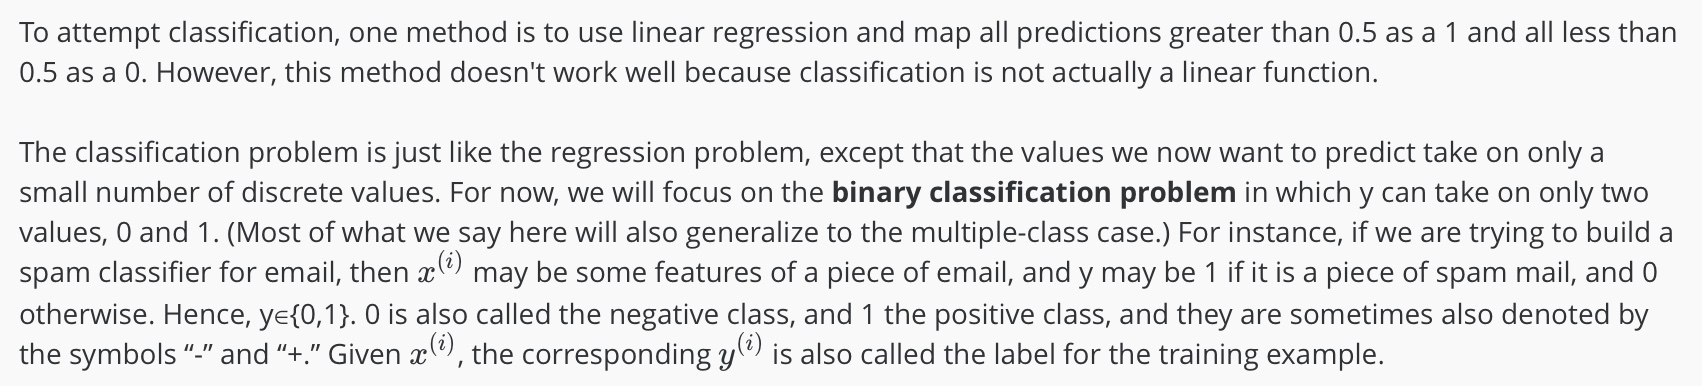
\includegraphics[width=1\textwidth]{./Imagenes/class1}
\end{figure}

\begin{figure}[H]
	\centering
	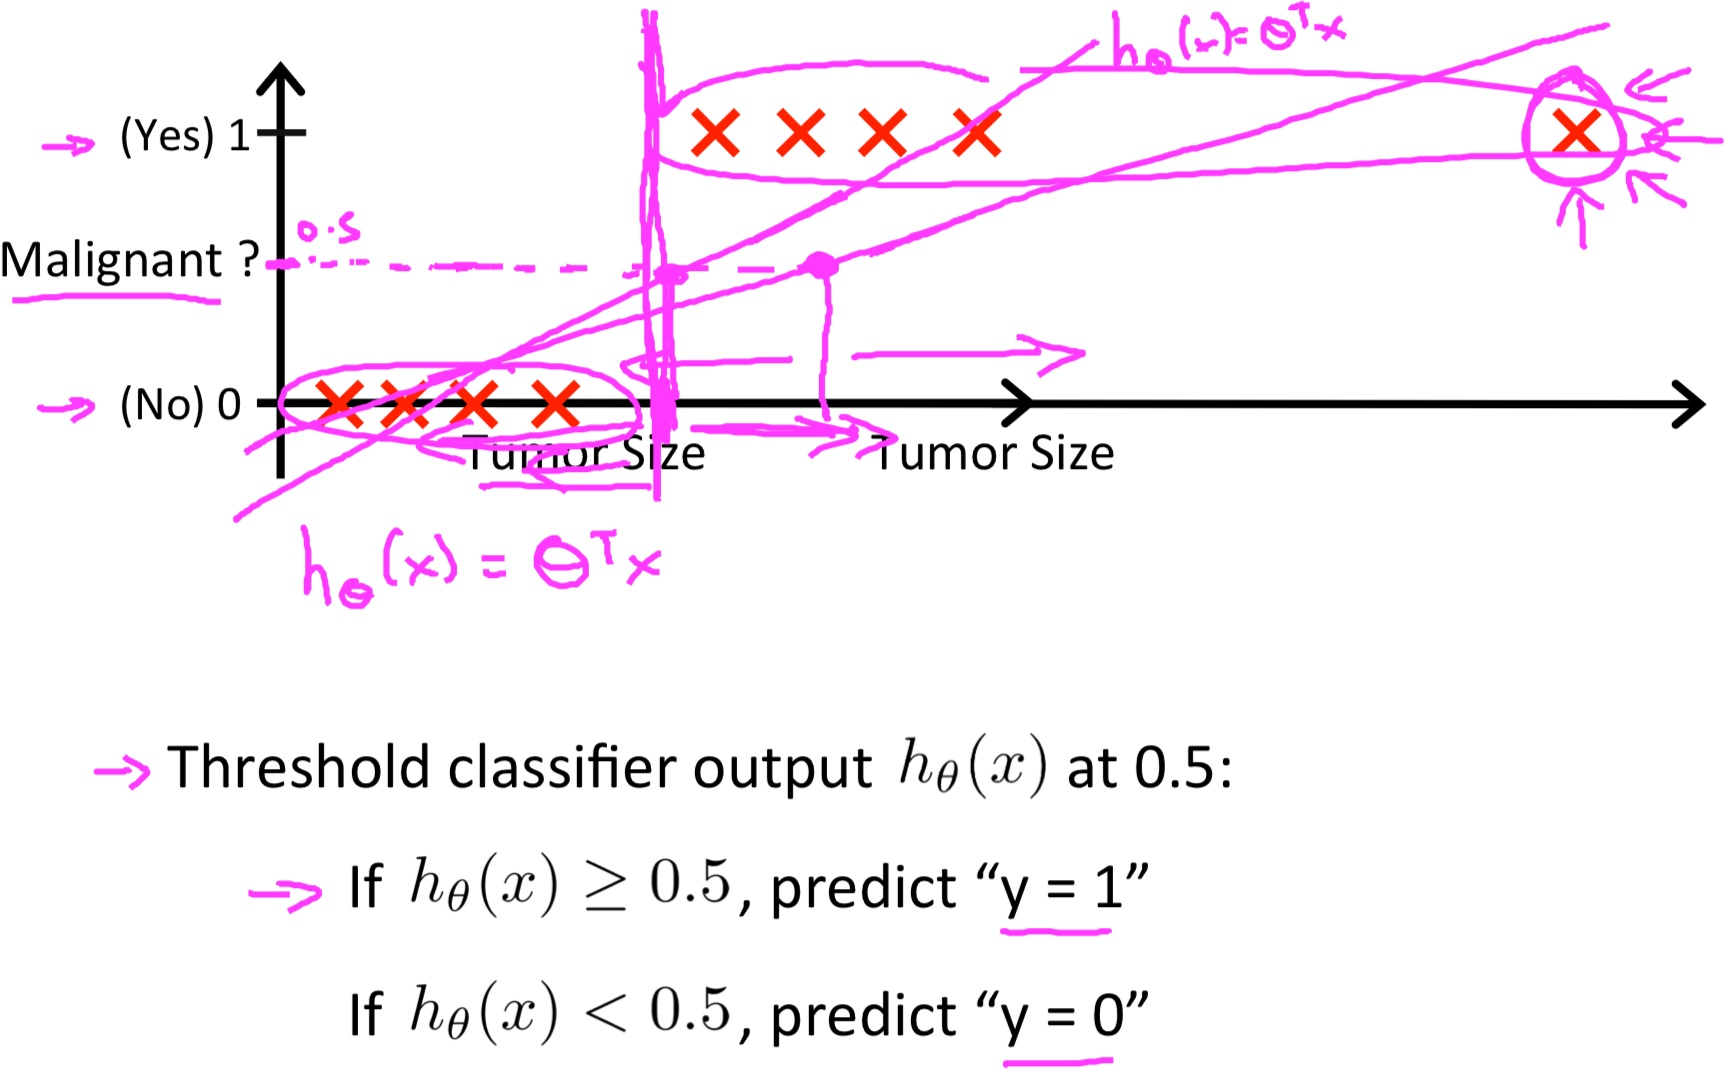
\includegraphics[width=1\textwidth]{./Imagenes/class2}
\end{figure}

\begin{figure}[H]
	\centering
	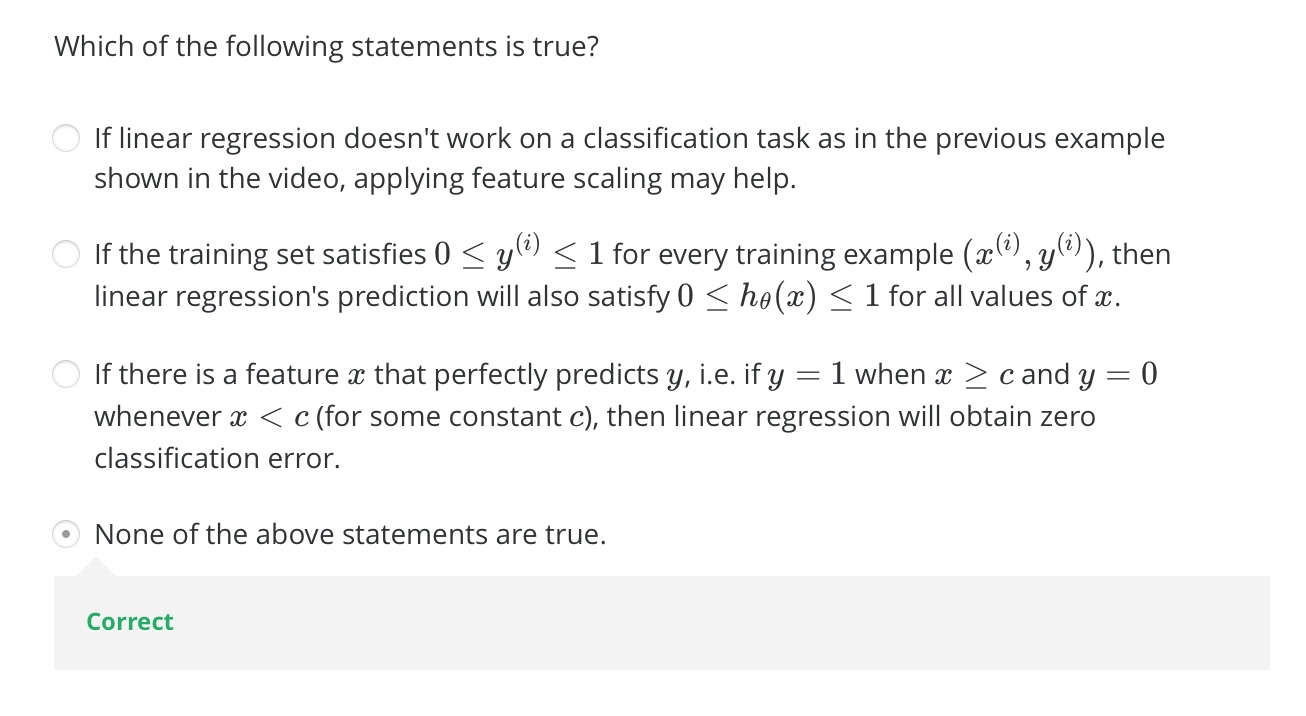
\includegraphics[width=1\textwidth]{./Imagenes/testClass}
\end{figure}
\newpage
\subsubsection{Hipothesis representation}
\begin{figure}[H]
	\centering
	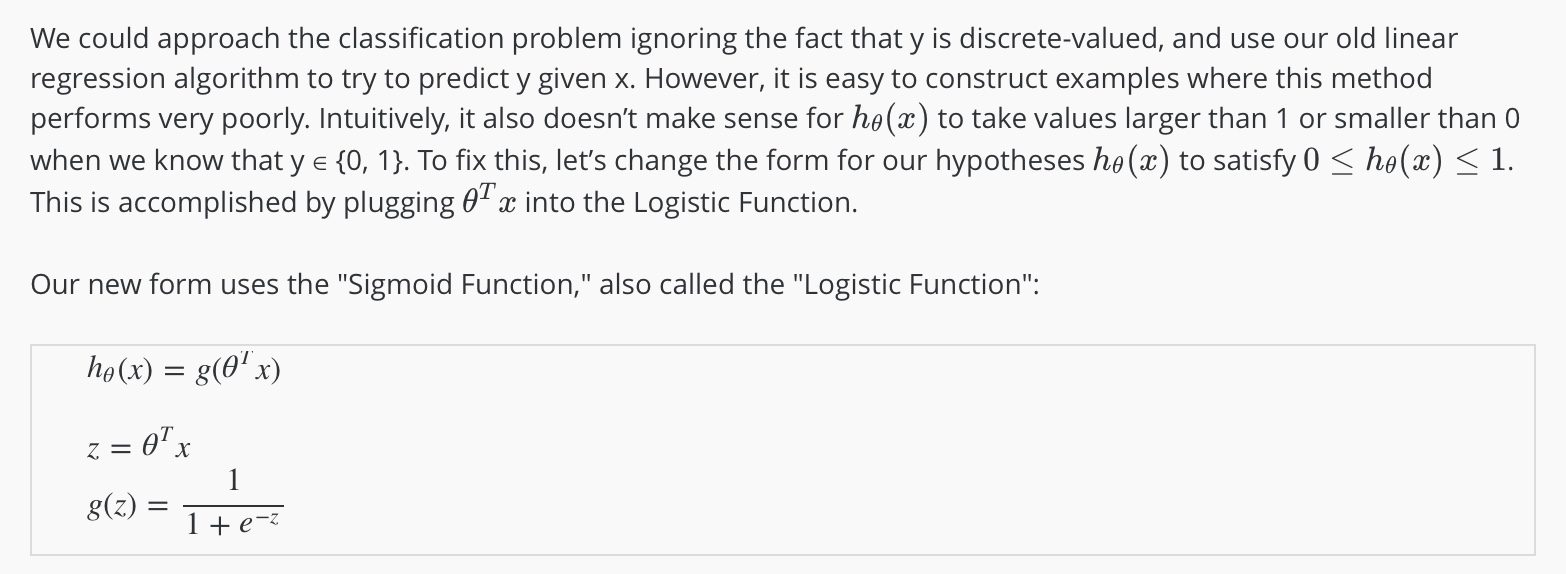
\includegraphics[width=1\textwidth]{./Imagenes/hipoRep1}
\end{figure}

\begin{figure}[H]
	\centering
	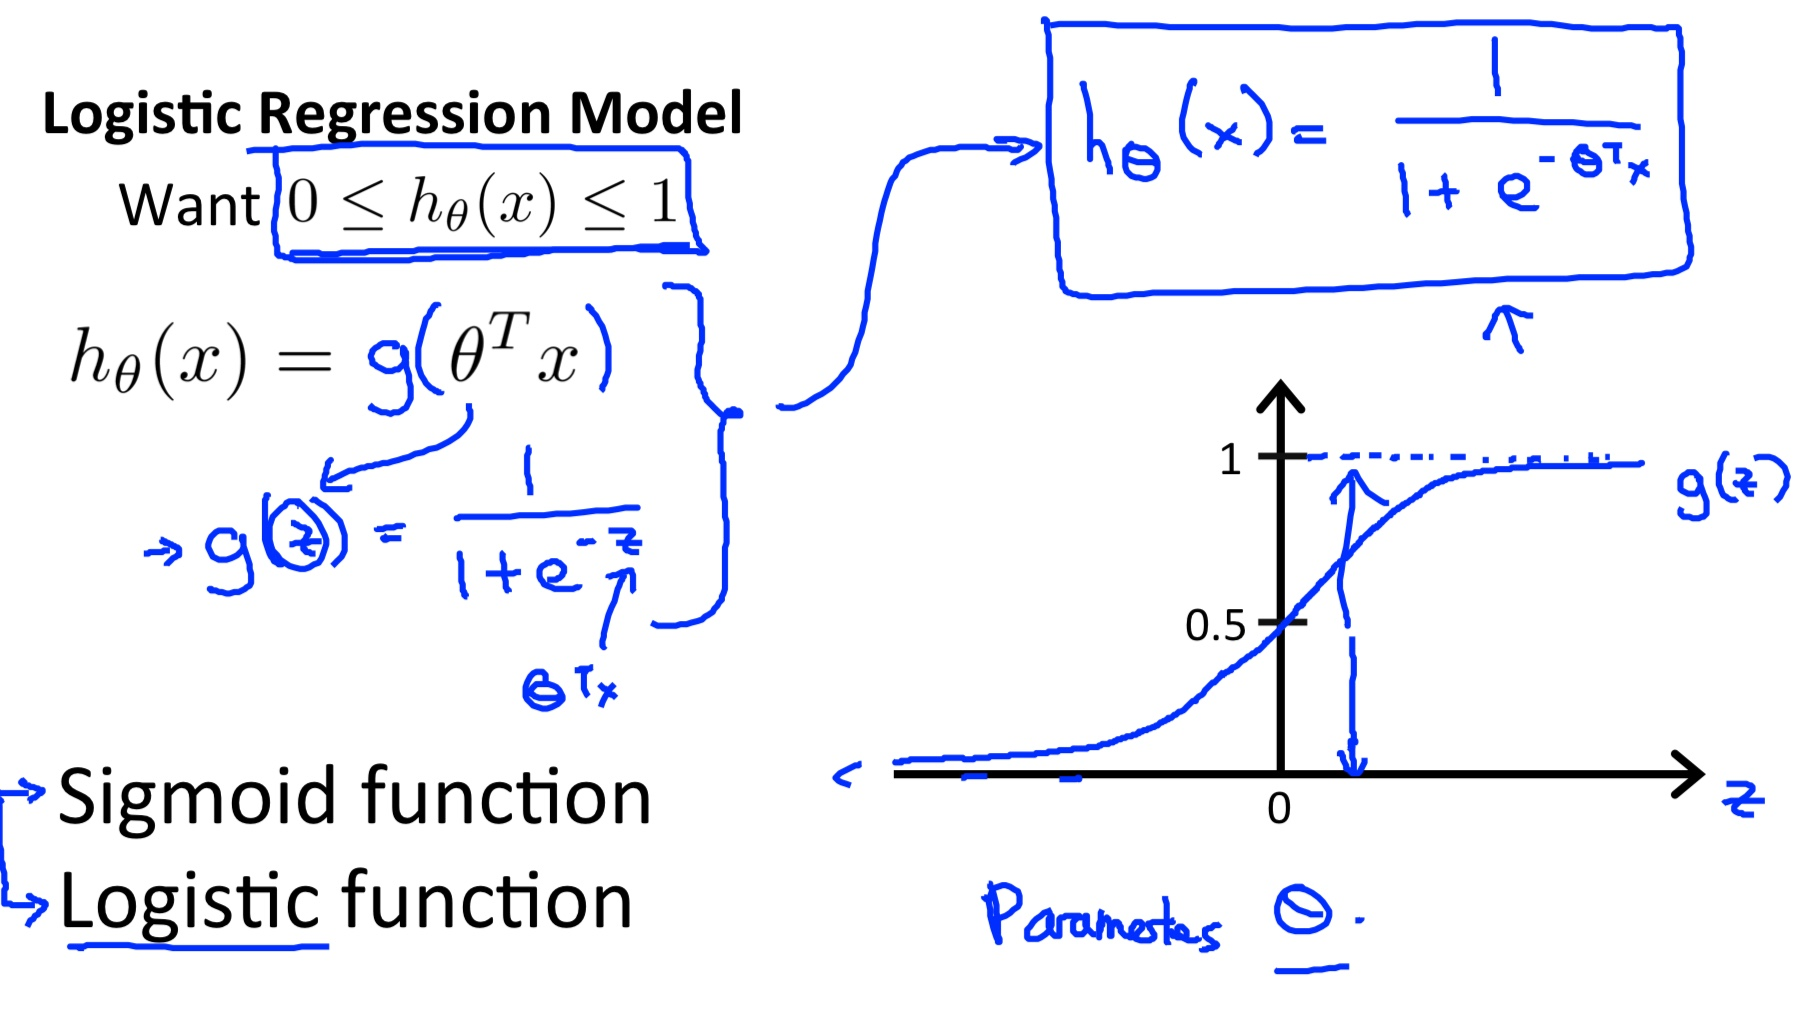
\includegraphics[width=1\textwidth]{./Imagenes/class3}
\end{figure}


\begin{figure}[H]
	\centering
	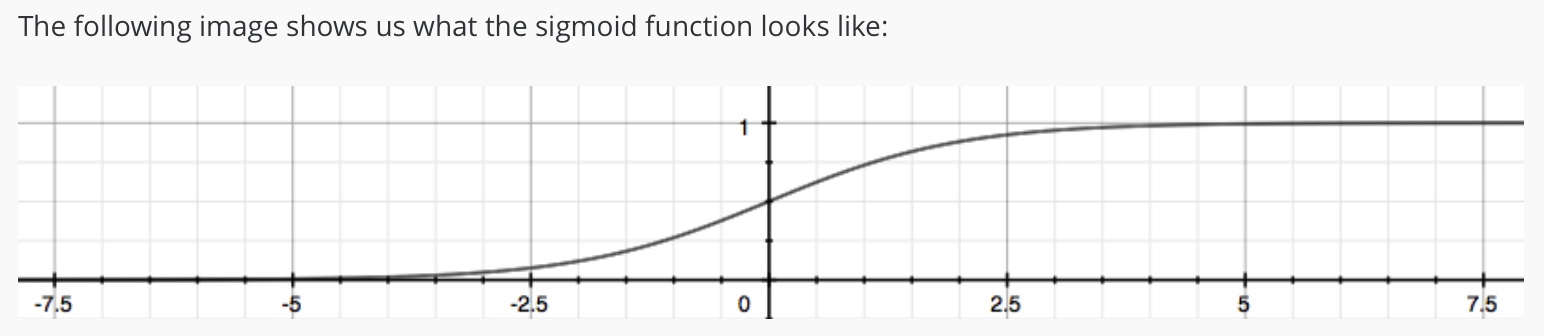
\includegraphics[width=1\textwidth]{./Imagenes/hipoRep2}
\end{figure}

\begin{figure}[H]
	\centering
	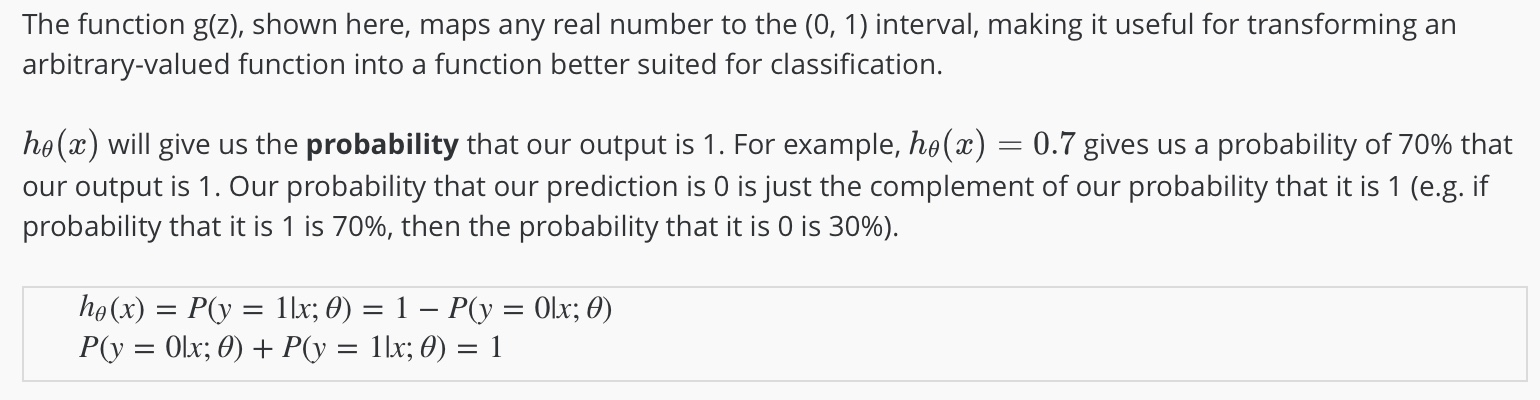
\includegraphics[width=1\textwidth]{./Imagenes/hipoRep3}
\end{figure}

\begin{figure}[H]
	\centering
	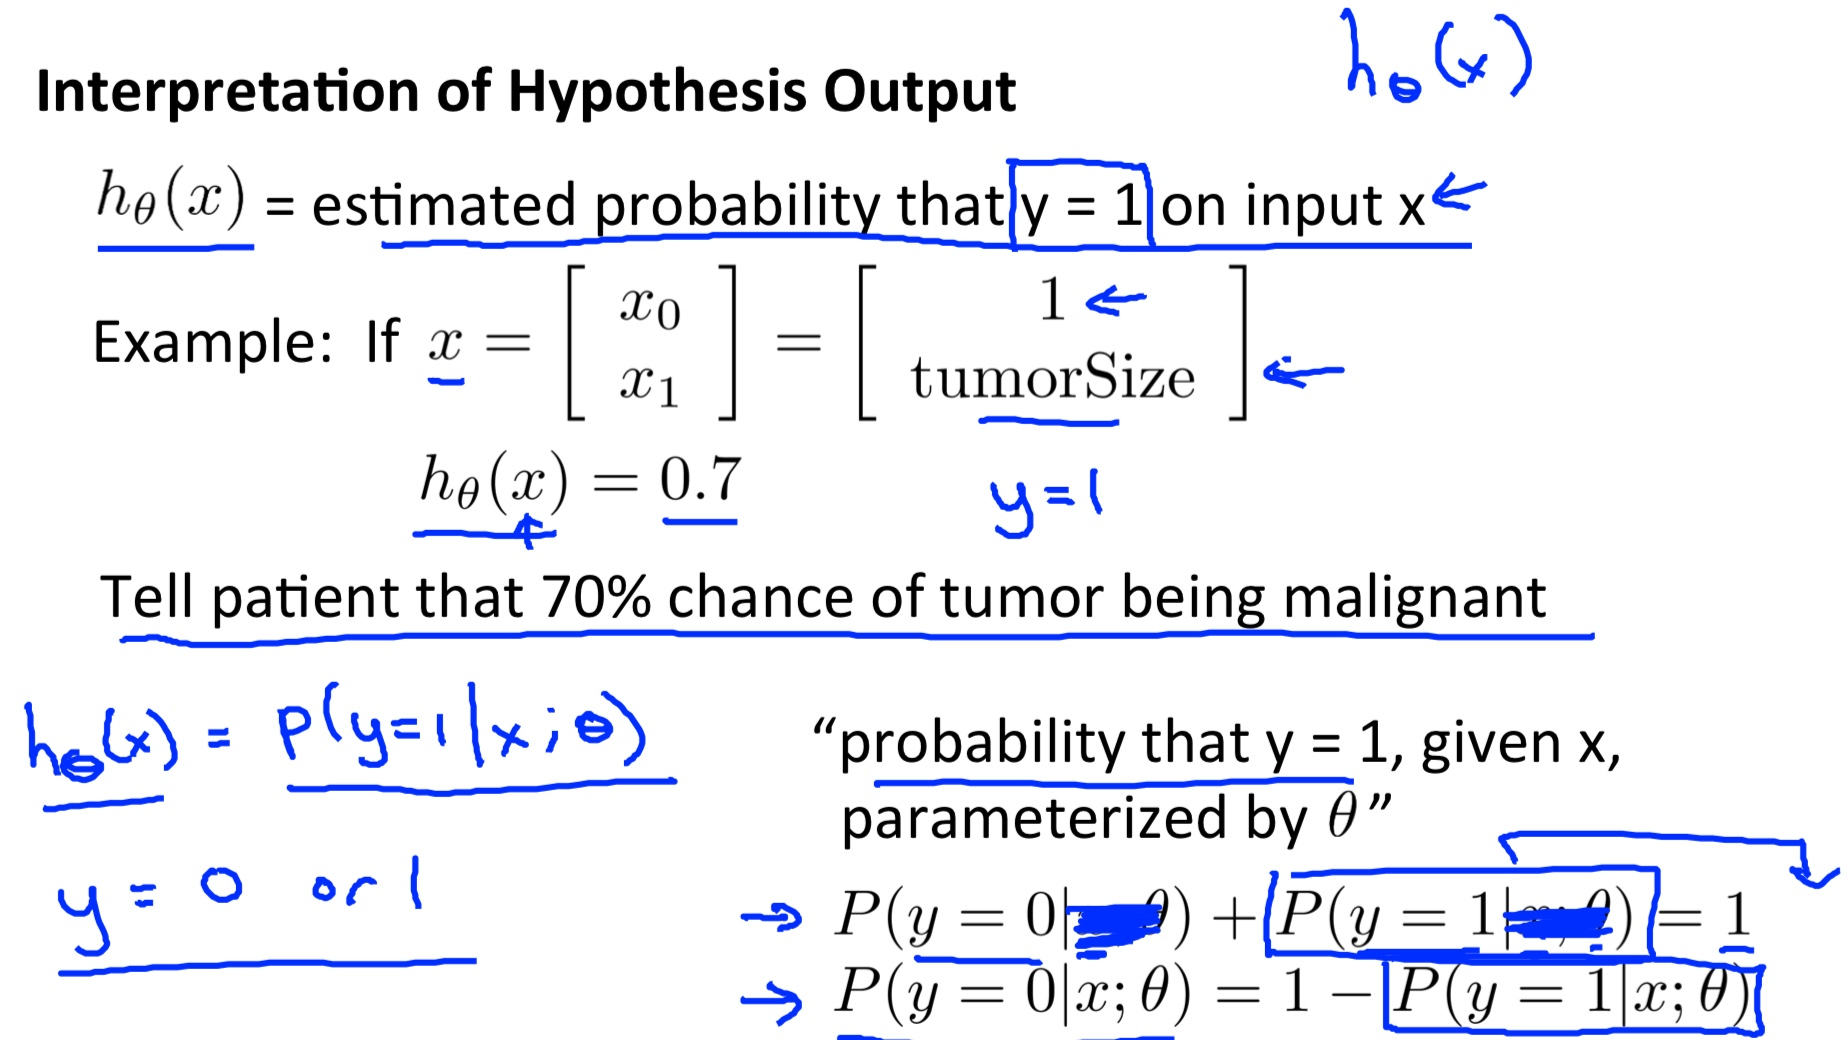
\includegraphics[width=1\textwidth]{./Imagenes/hipoRep4}
\end{figure}
\begin{figure}[H]
	\centering
	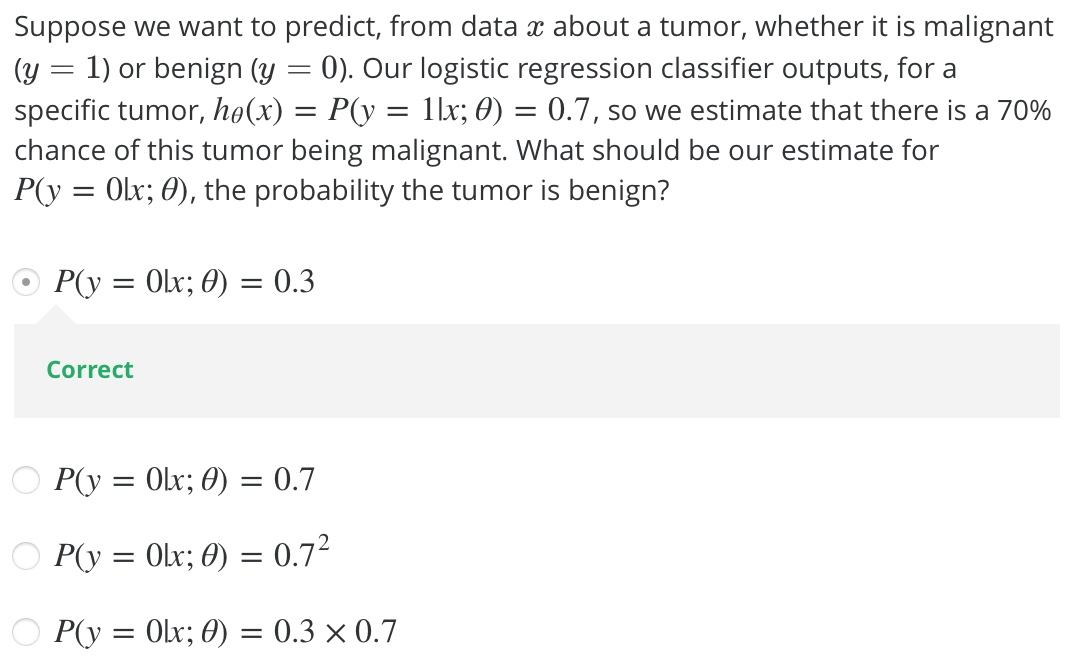
\includegraphics[width=1\textwidth]{./Imagenes/testHipo}
\end{figure}
\newpage
\subsubsection{Decision boundary}

\begin{figure}[H]
	\centering
	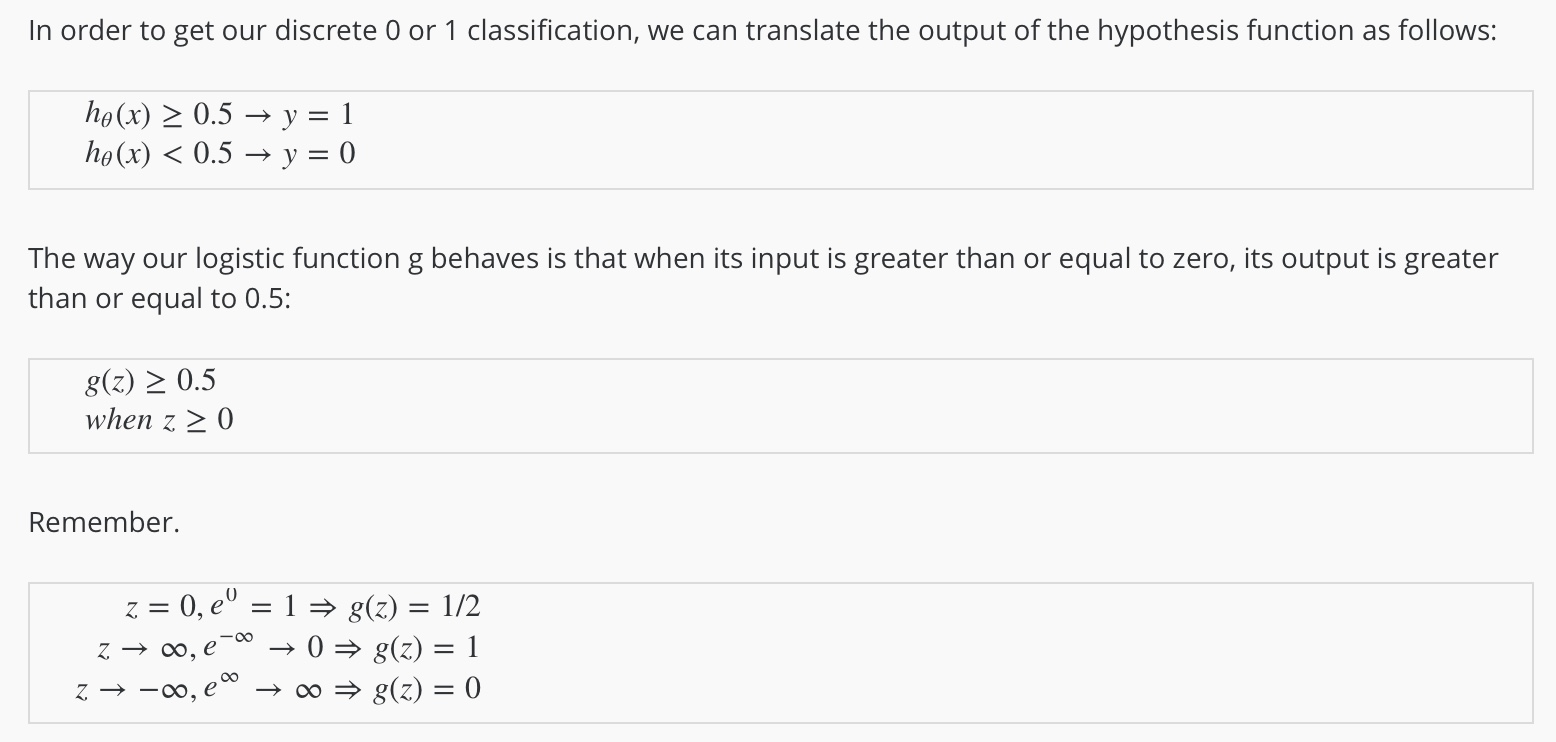
\includegraphics[width=1\textwidth]{./Imagenes/decBound1}
\end{figure}

\begin{figure}[H]
	\centering
	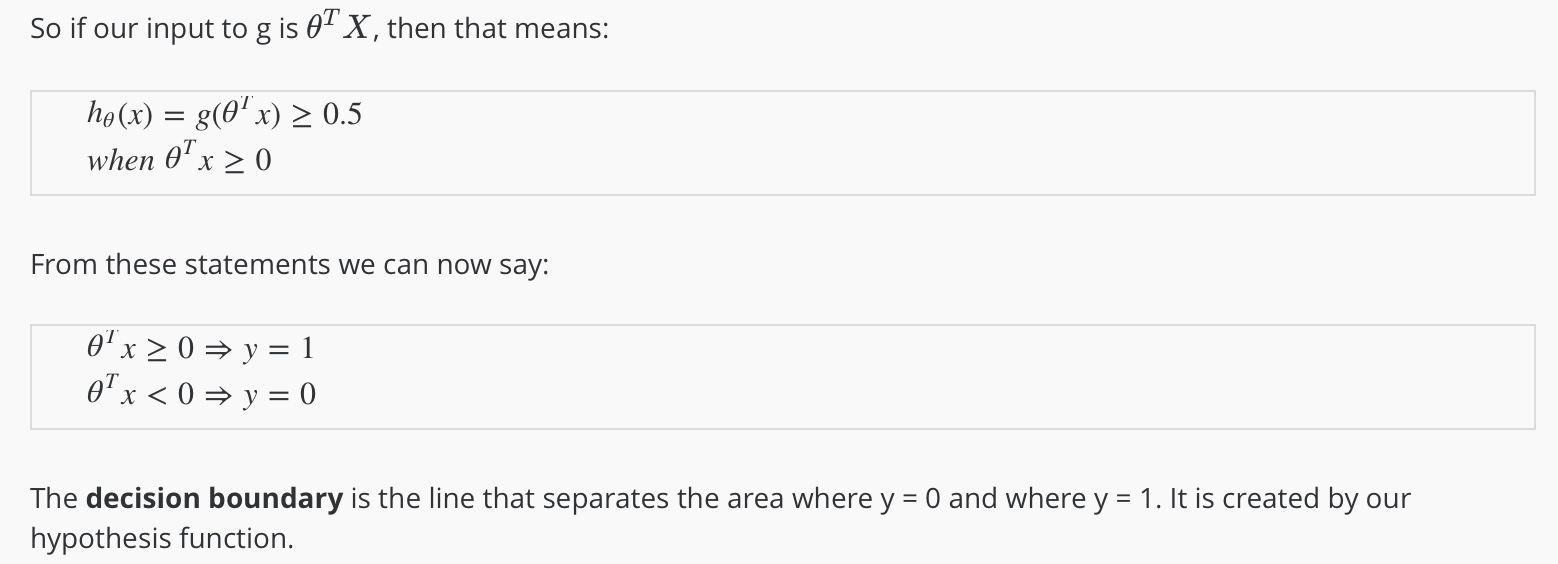
\includegraphics[width=1\textwidth]{./Imagenes/decBound2}
\end{figure}

\begin{figure}[H]
	\centering
	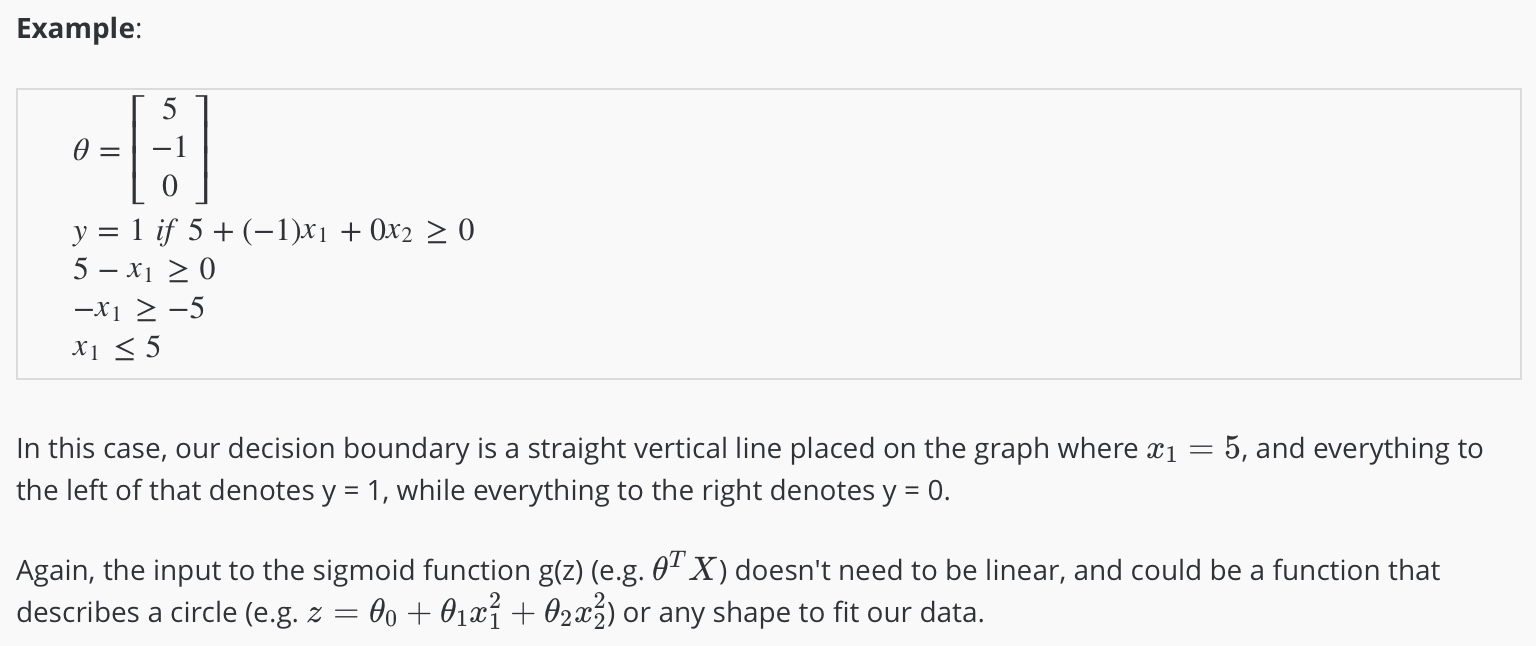
\includegraphics[width=0.9\textwidth]{./Imagenes/decBound3}
\end{figure}

\begin{figure}[H]
	\centering
	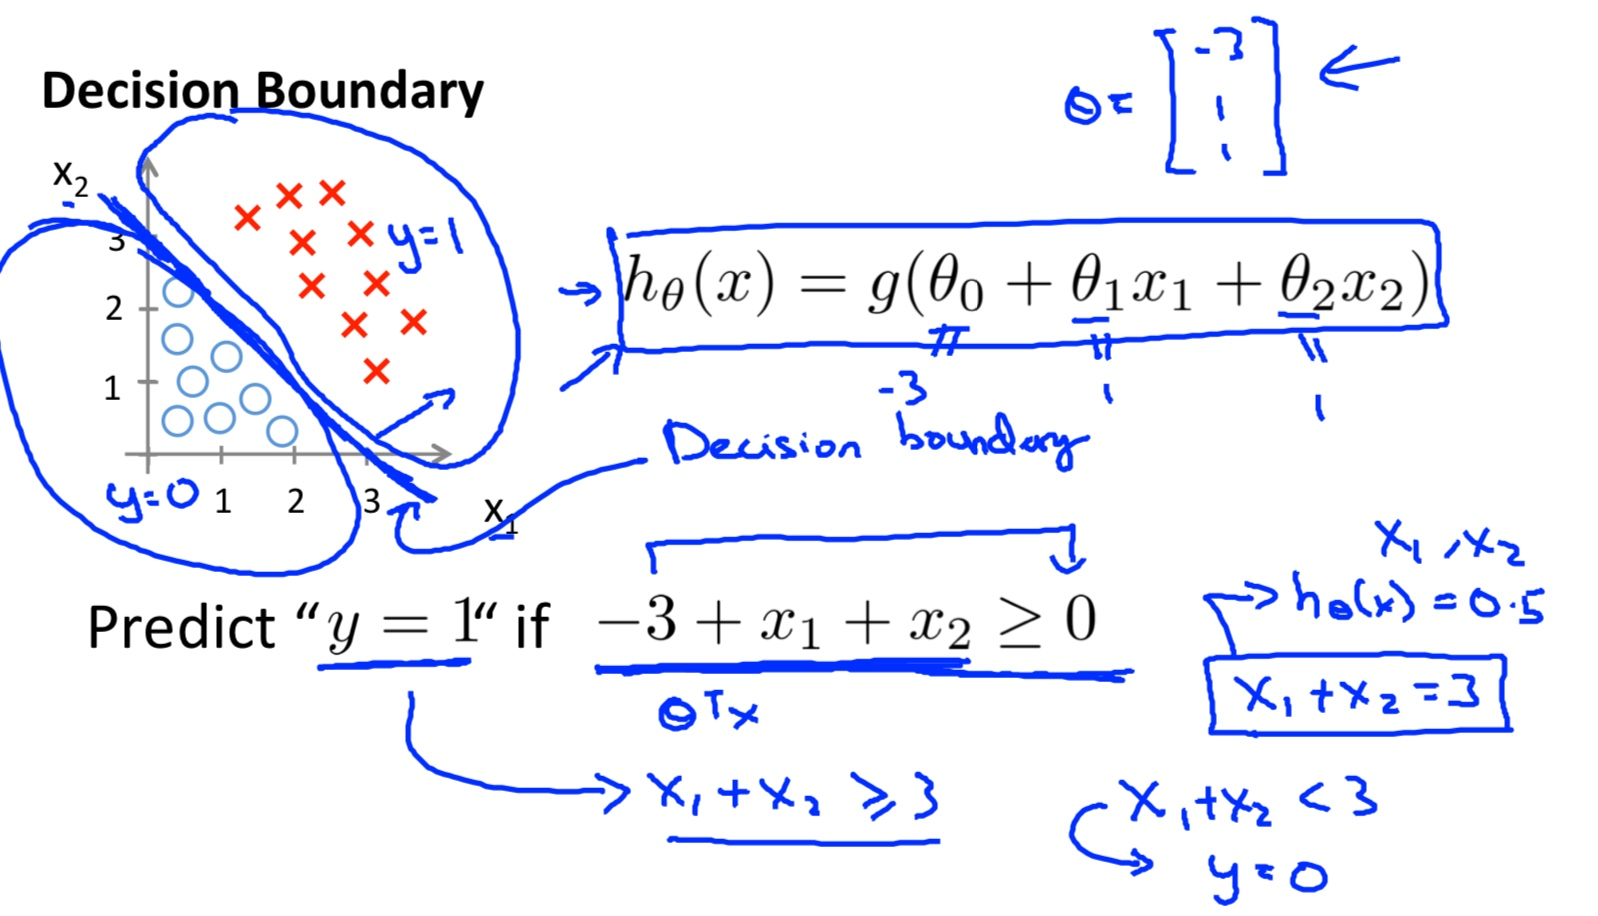
\includegraphics[width=1\textwidth]{./Imagenes/decBound4}
\end{figure}

\begin{figure}[H]
	\centering
	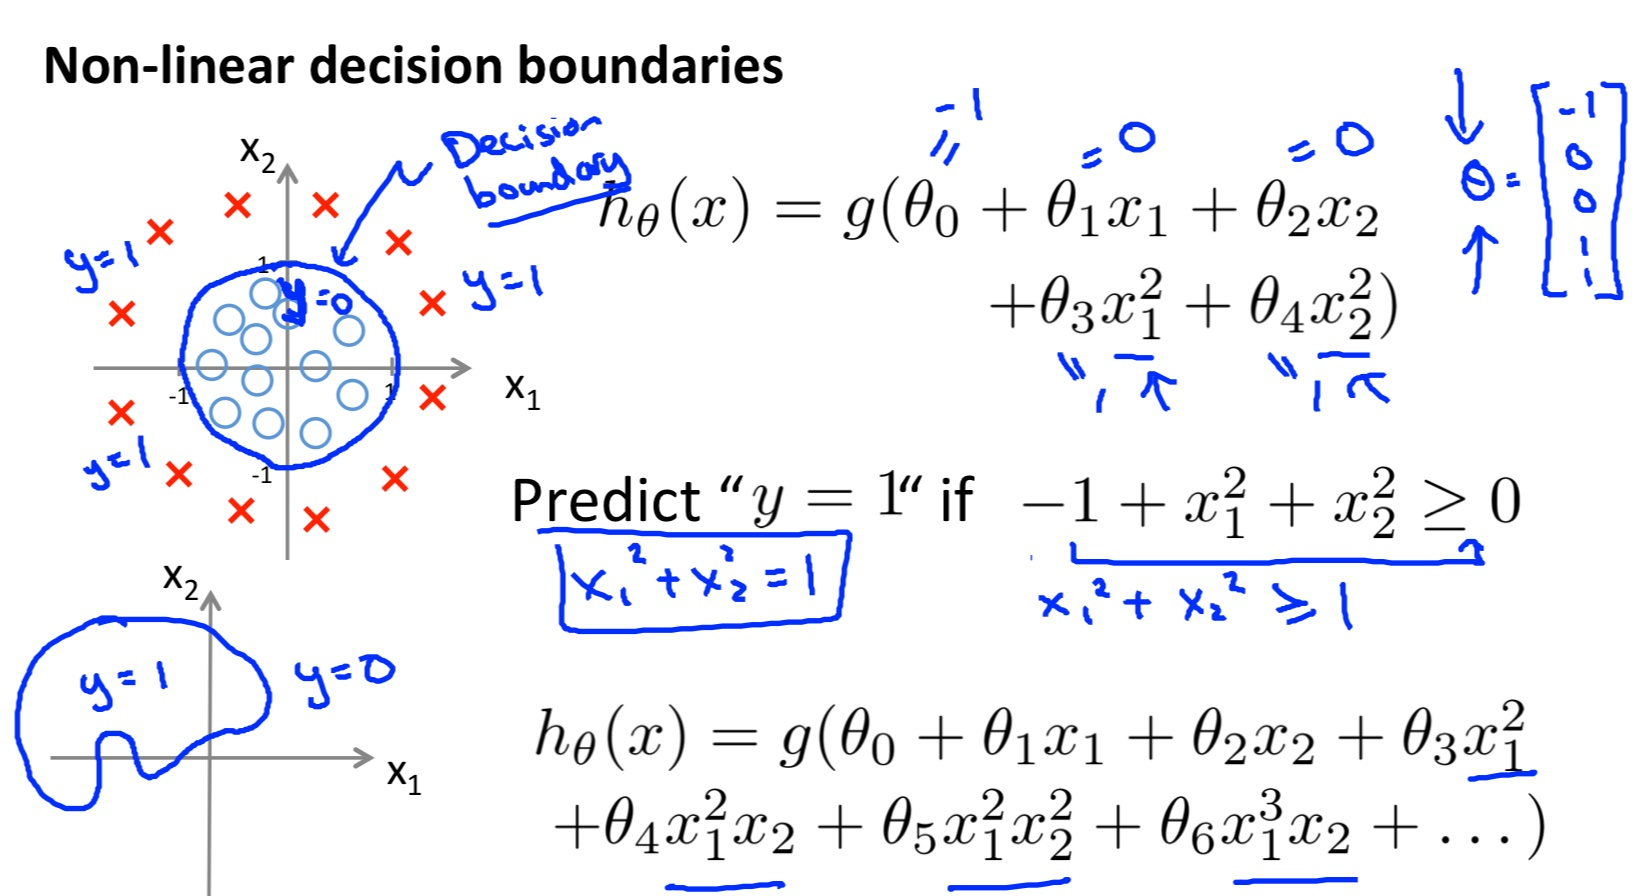
\includegraphics[width=1\textwidth]{./Imagenes/decBound5}
\end{figure}
\begin{figure}[H]
	\centering
	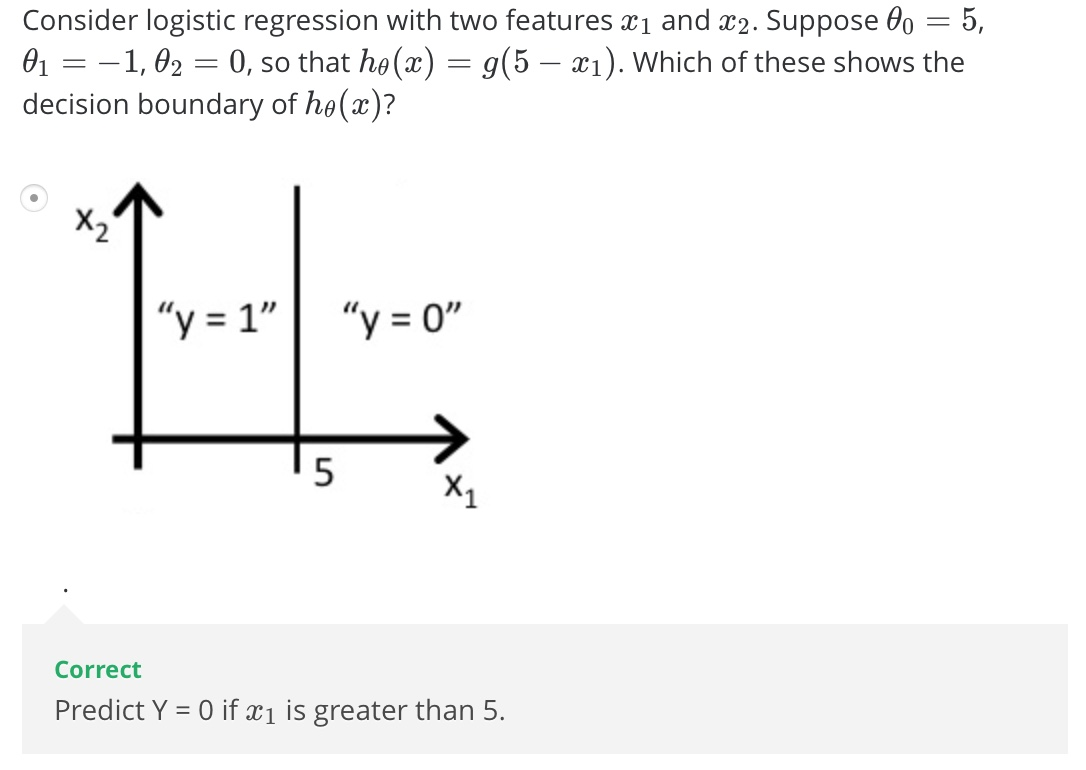
\includegraphics[width=1\textwidth]{./Imagenes/testDecbound}
\end{figure}

\newpage

\subsection{Logistic Regression Model}
\subsubsection{Cost Function}

\begin{figure}[H]
	\centering
	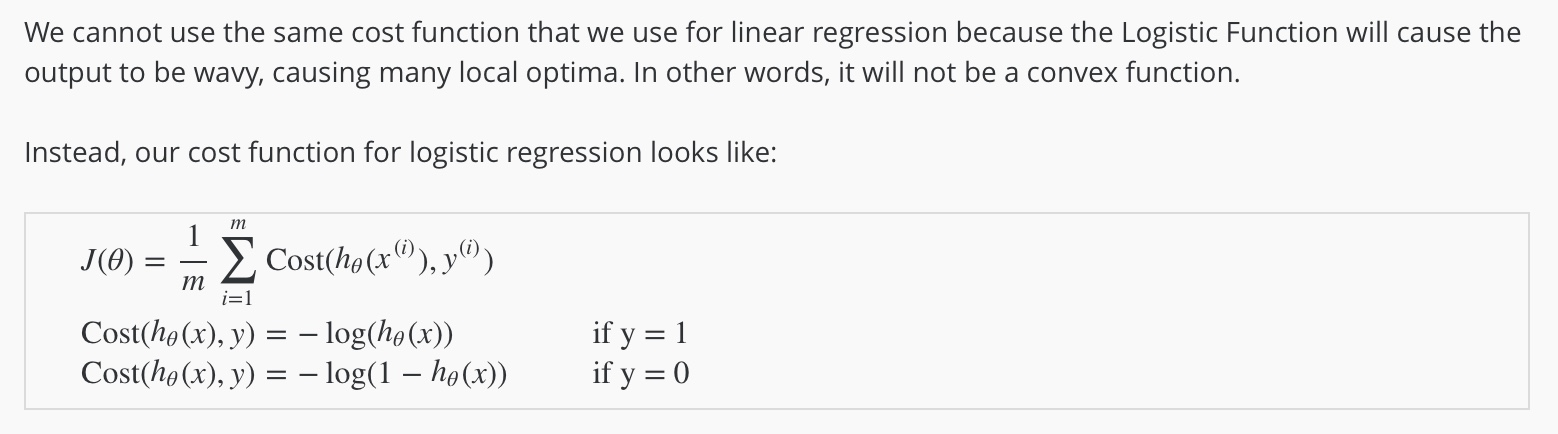
\includegraphics[width=1\textwidth]{./Imagenes/costFunc1}
\end{figure}


\begin{figure}[H]
\minipage{0.5\textwidth}
  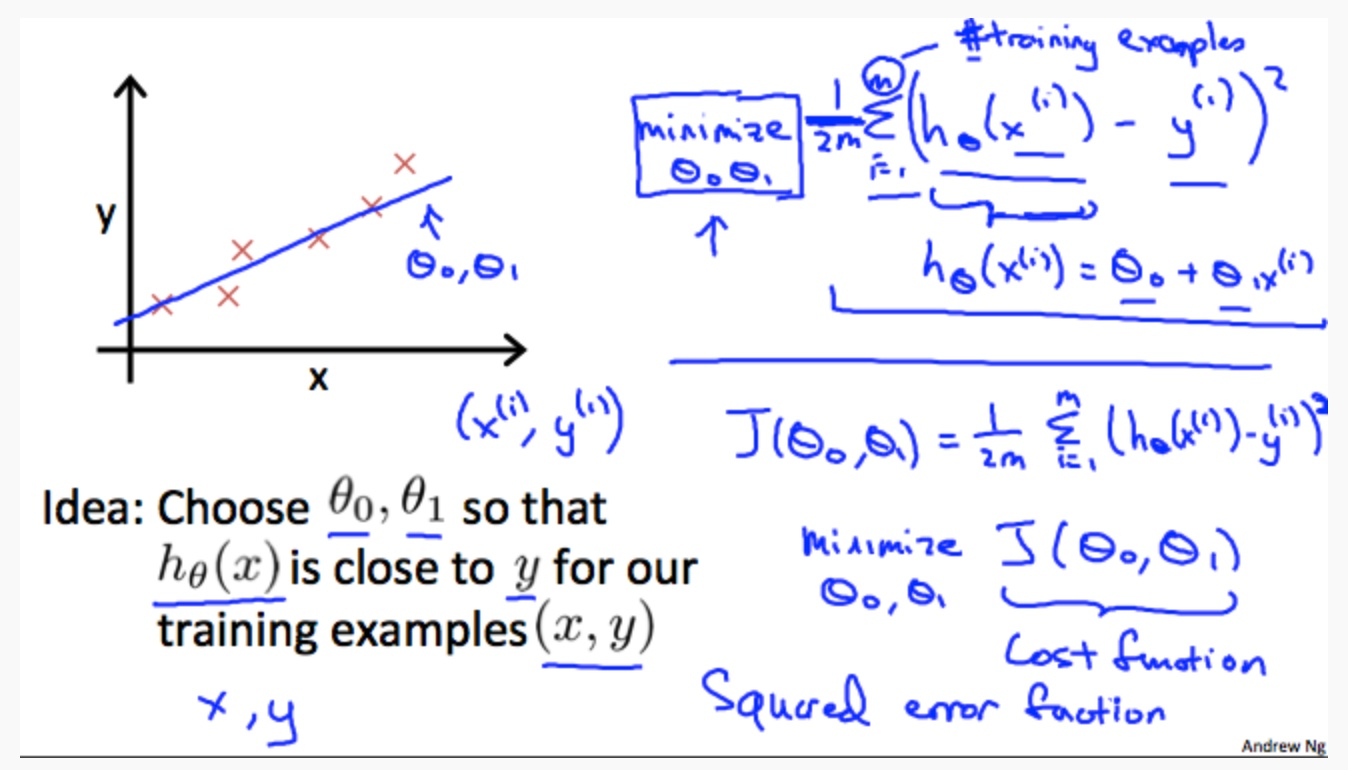
\includegraphics[width=\linewidth]{./Imagenes/costFunc2}
\endminipage\hfill
\minipage{0.525\textwidth}
  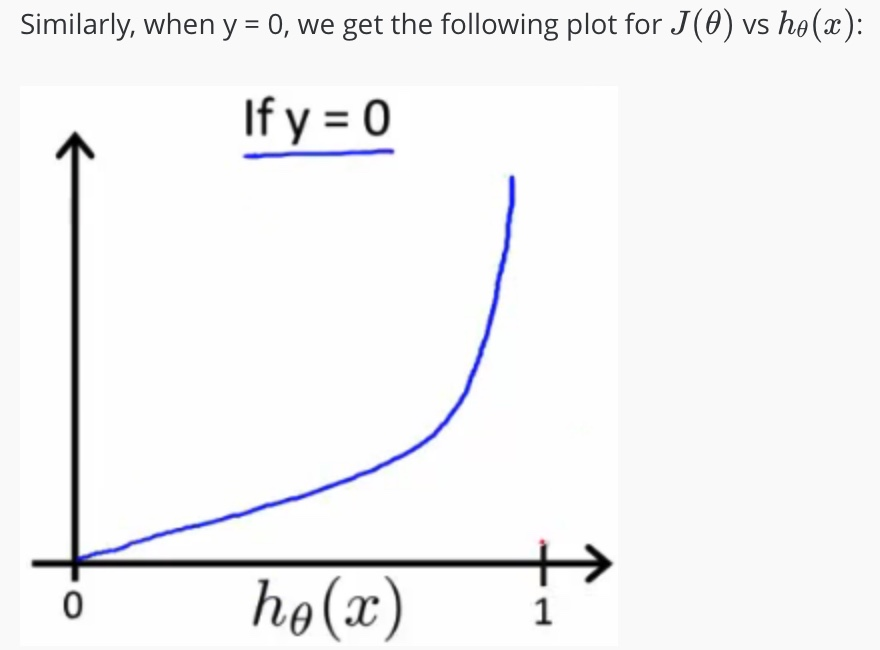
\includegraphics[width=\linewidth]{./Imagenes/costFunc3}
\endminipage\hfill
\end{figure}

\begin{figure}[H]
	\centering
	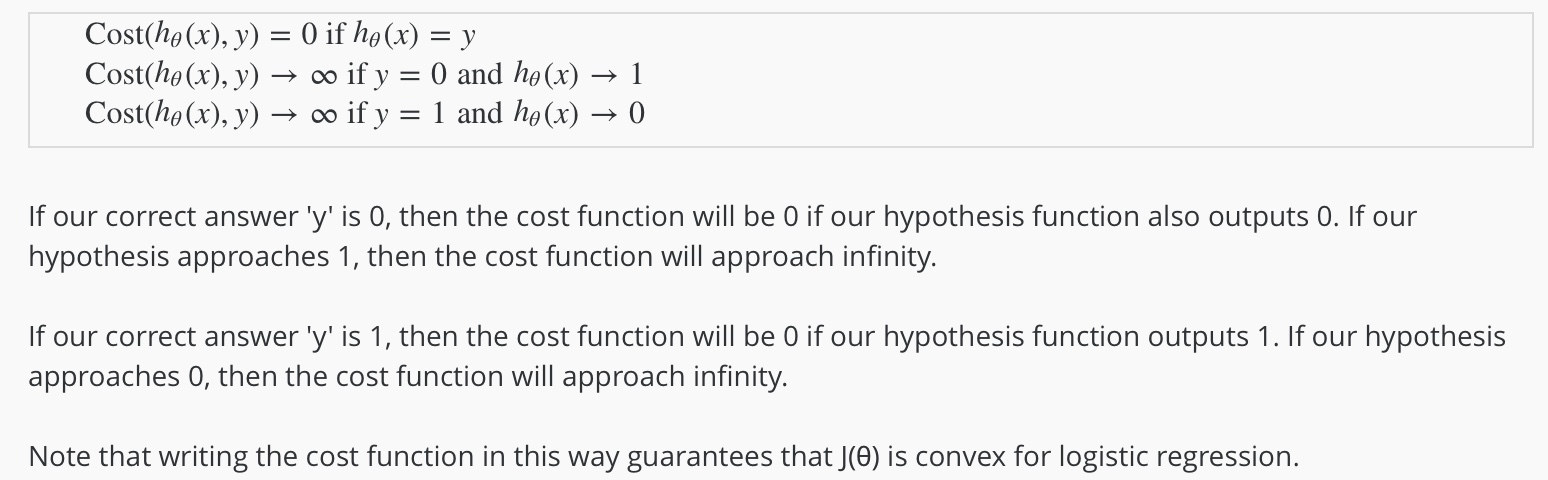
\includegraphics[width=1\textwidth]{./Imagenes/costFunc4}
\end{figure}

\begin{figure}[H]
	\centering
	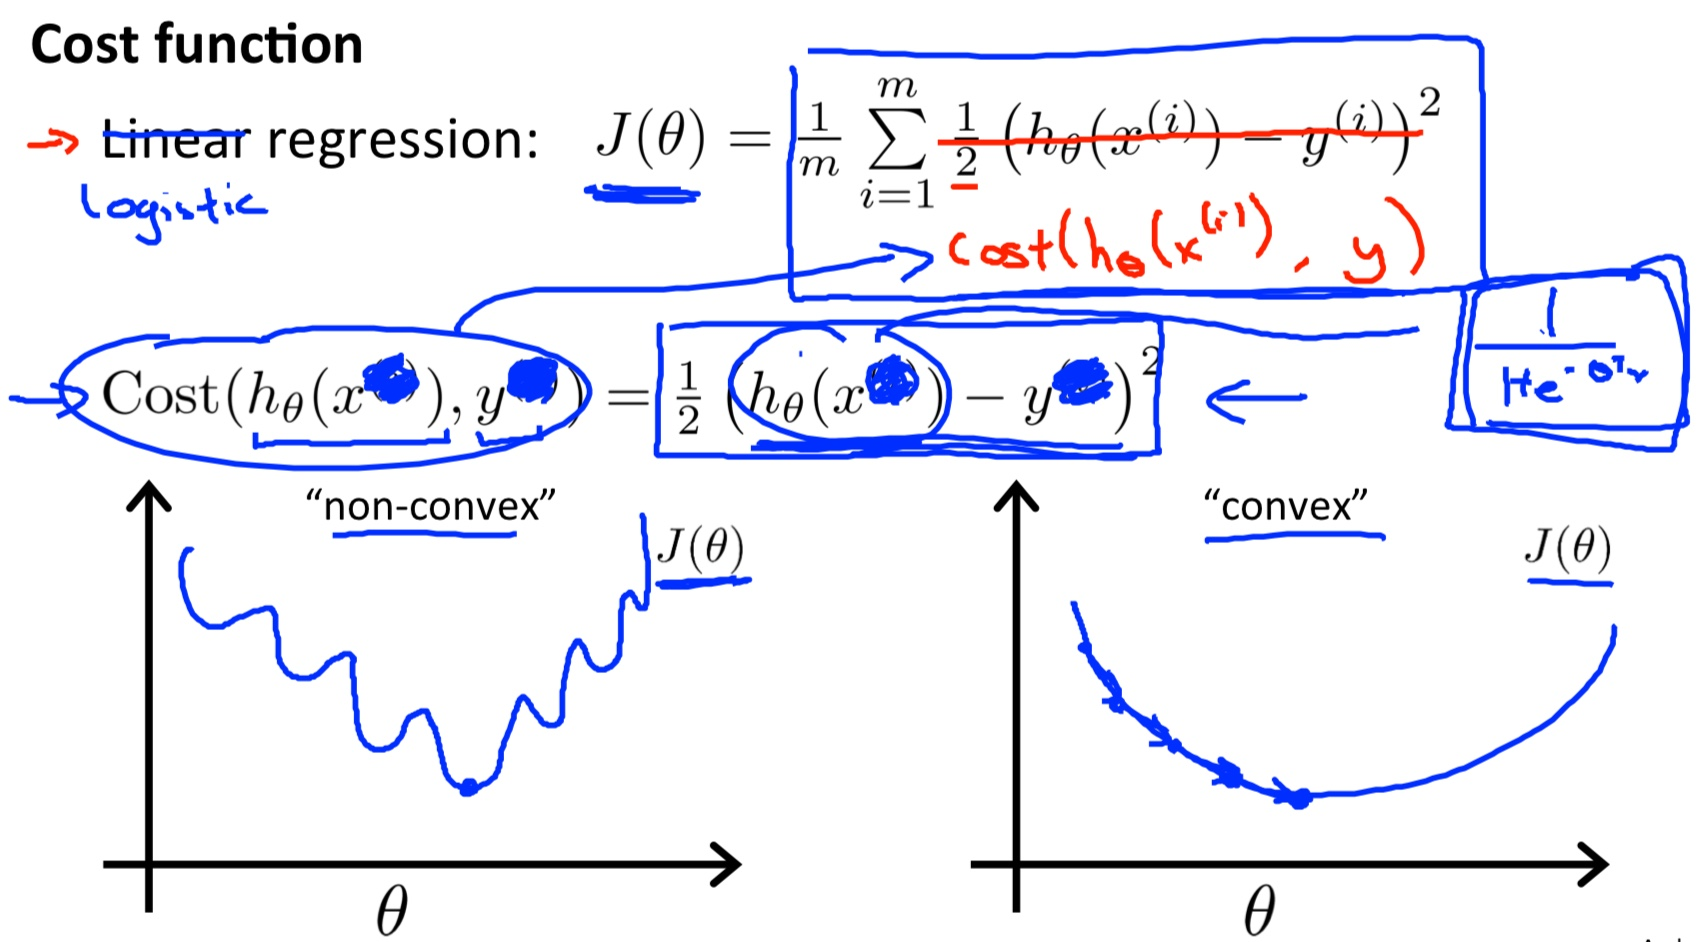
\includegraphics[width=1\textwidth]{./Imagenes/costFunc5}
\end{figure}

\begin{figure}[H]
	\centering
	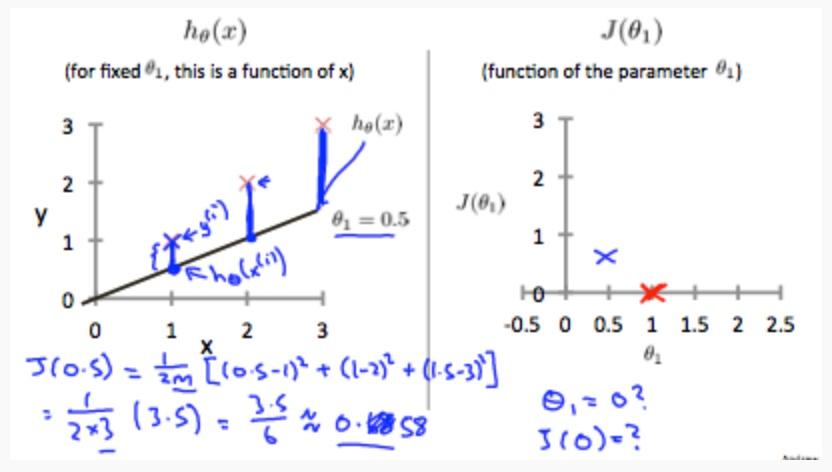
\includegraphics[width=1\textwidth]{./Imagenes/costFunc6}
\end{figure}

\begin{figure}[H]
	\centering
	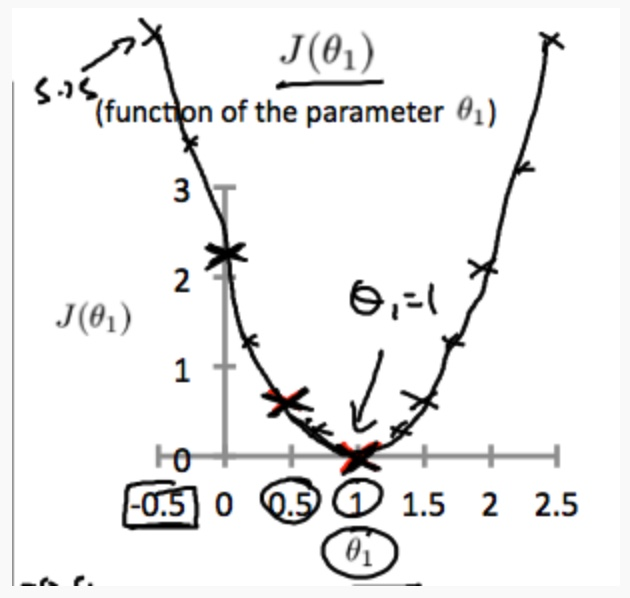
\includegraphics[width=0.8\textwidth]{./Imagenes/costFunc7}
\end{figure}

\begin{figure}[H]
	\centering
	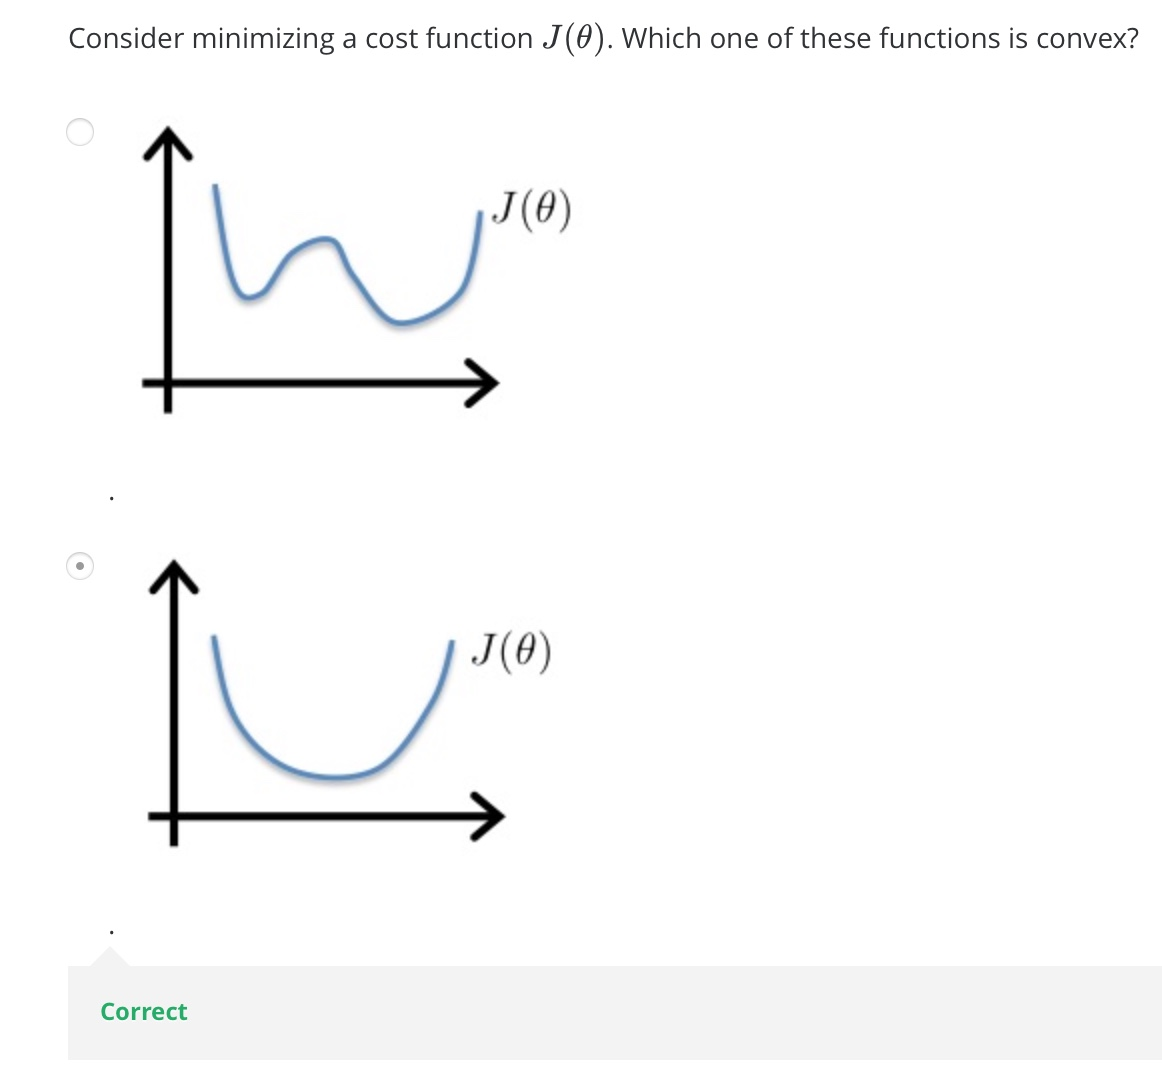
\includegraphics[width=0.8\textwidth]{./Imagenes/testCostFunc1}
\end{figure}

\begin{figure}[H]
	\centering
	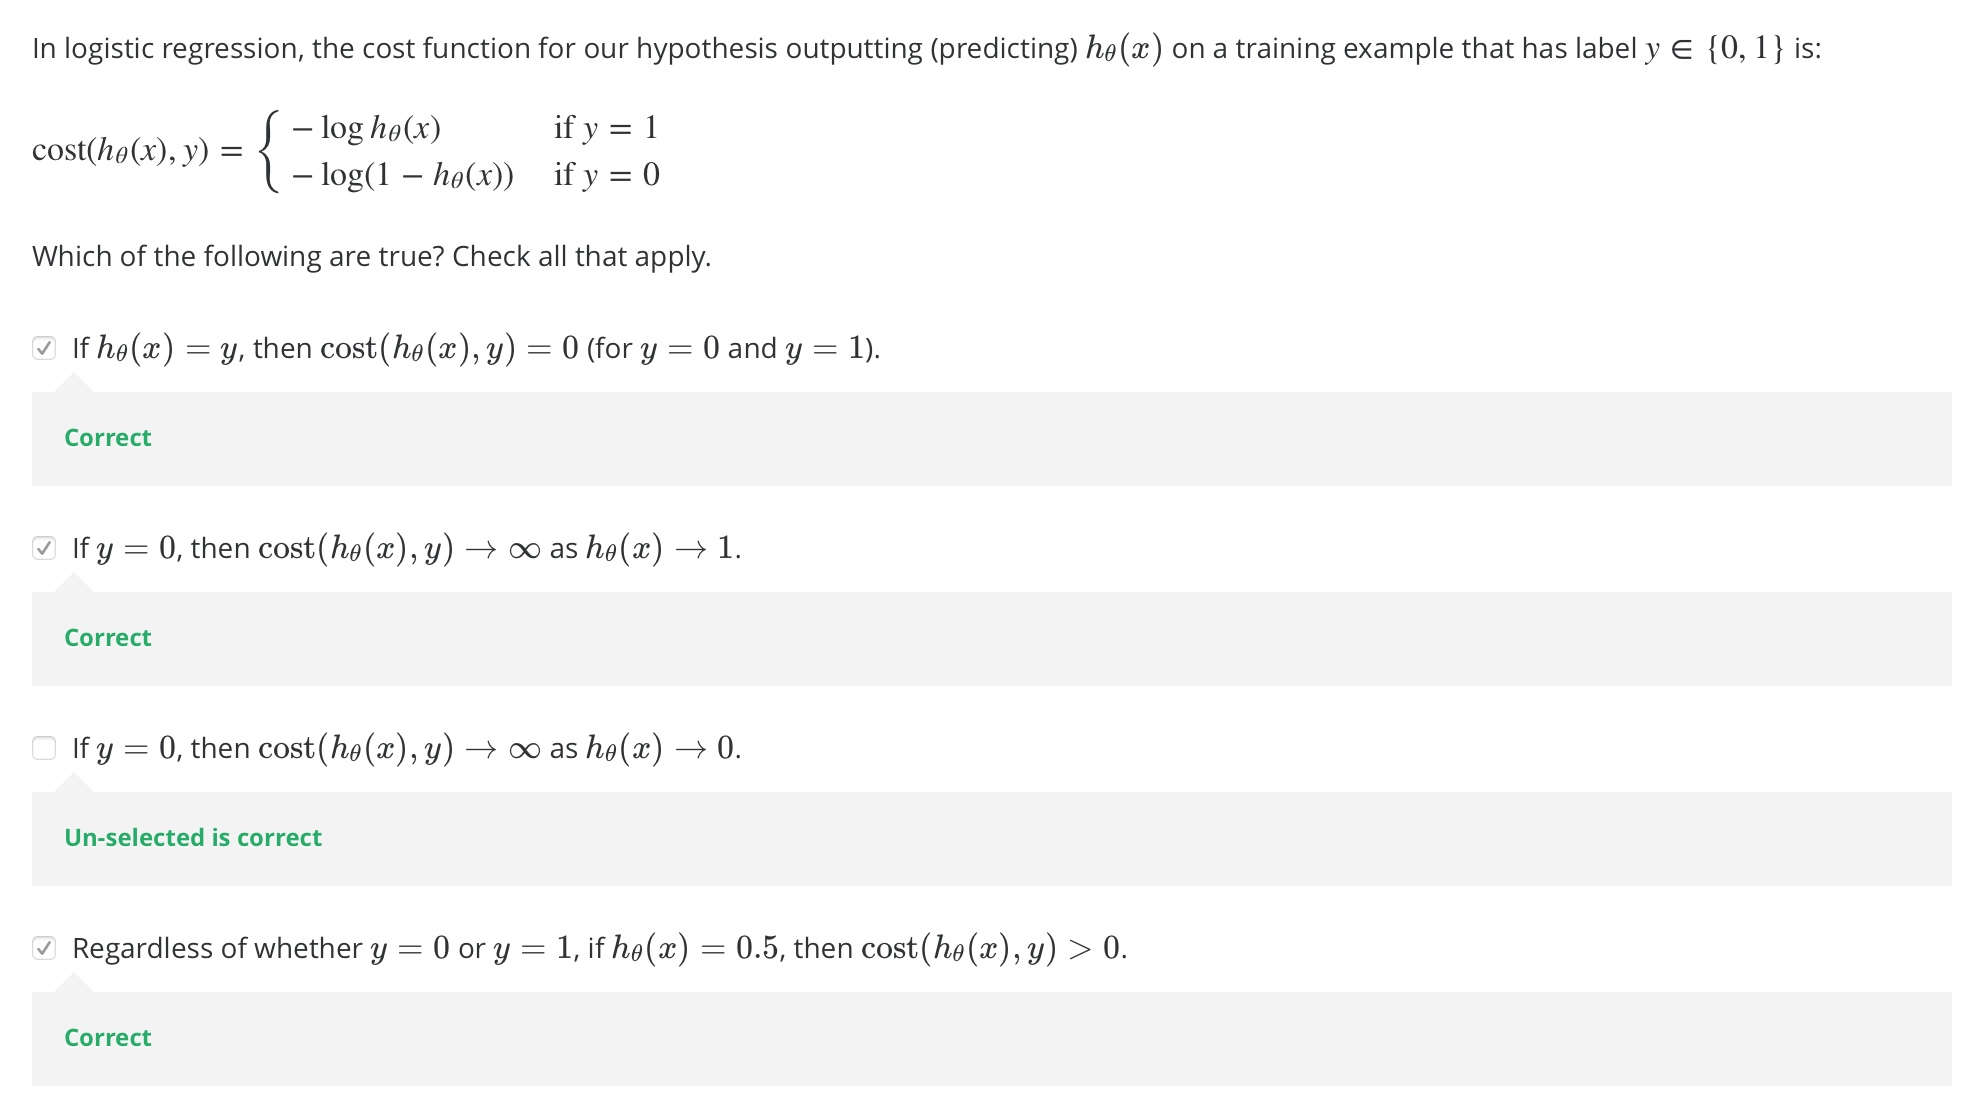
\includegraphics[width=1\textwidth]{./Imagenes/testCostFunc2}
\end{figure}

\newpage

\subsubsection{Simplified cost function}
\begin{figure}[H]
	\centering
	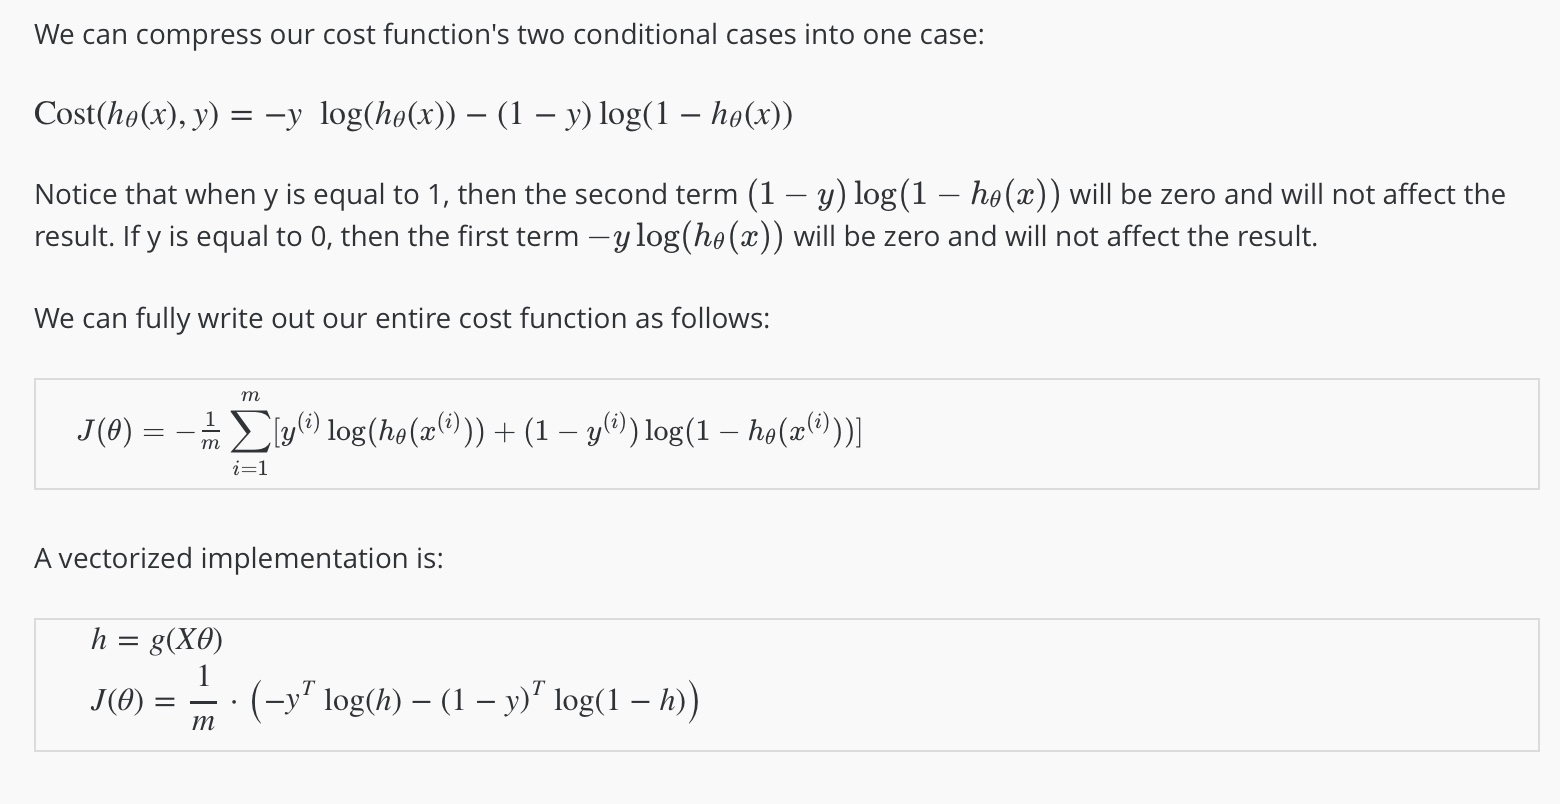
\includegraphics[width=1\textwidth]{./Imagenes/simpleCostFunc1}
\end{figure}

\begin{figure}[H]
	\centering
	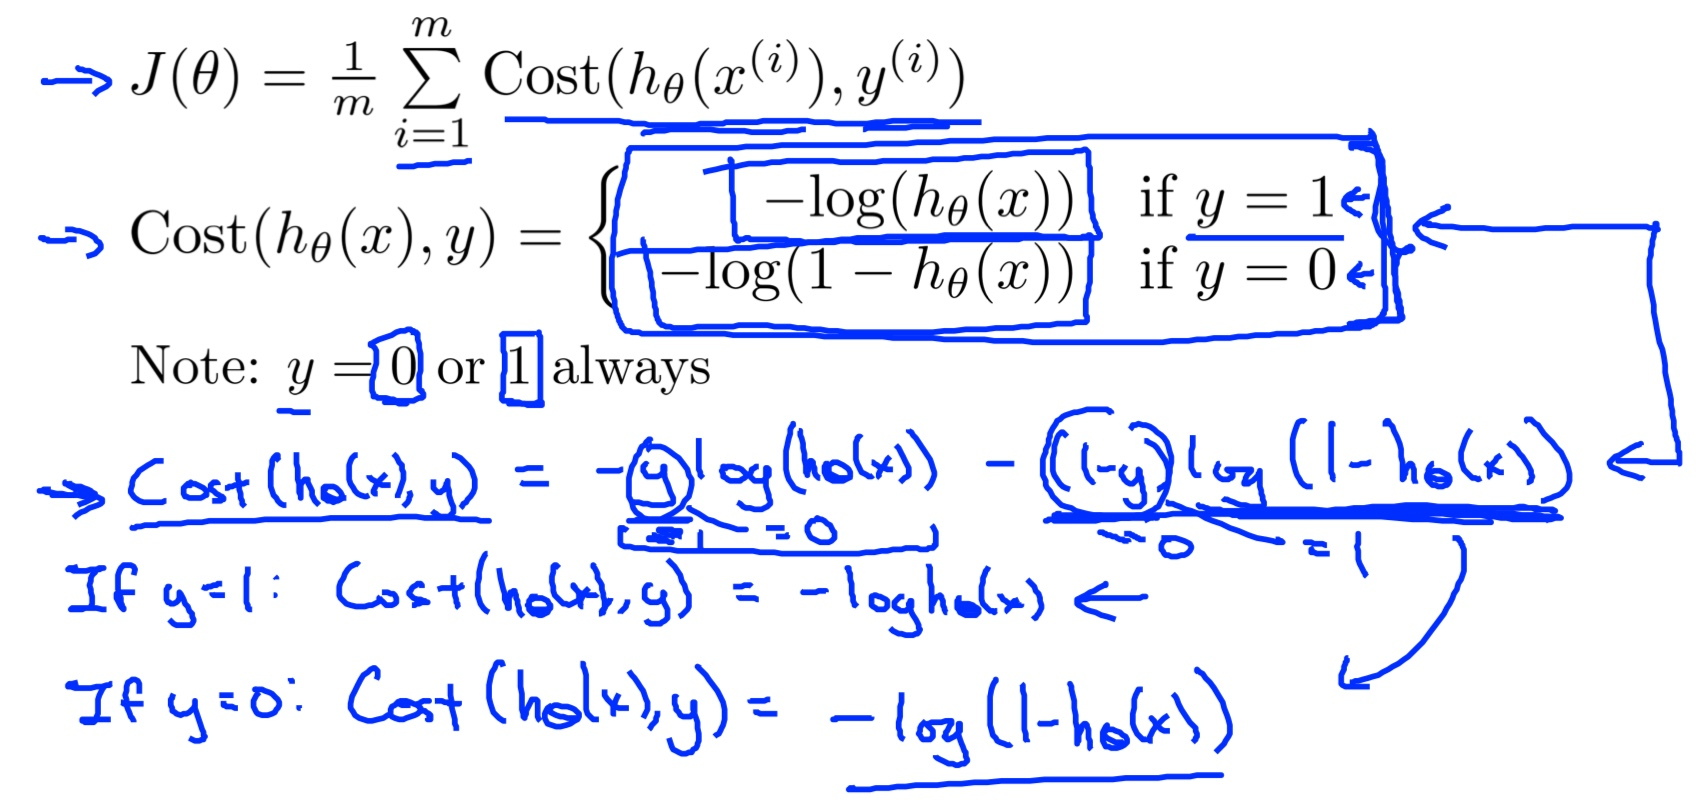
\includegraphics[width=1\textwidth]{./Imagenes/simpleCostFunc2}
\end{figure}

\begin{figure}[H]
	\centering
	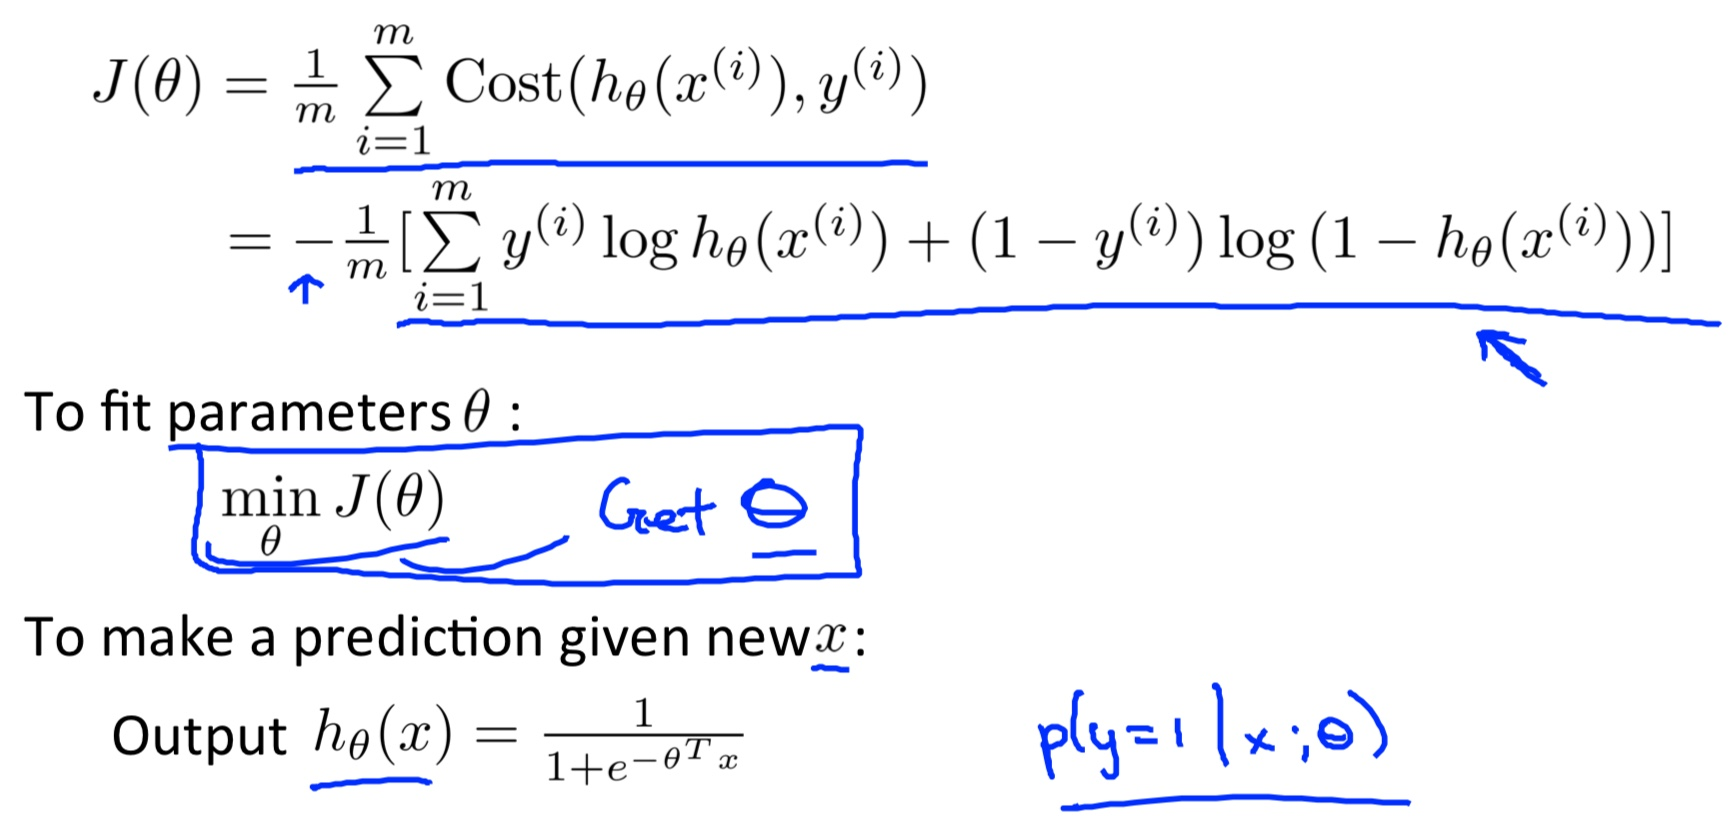
\includegraphics[width=1\textwidth]{./Imagenes/simpleCostFunc3}
\end{figure}

\subsubsection{Gradient descent}
\begin{figure}[H]
	\centering
	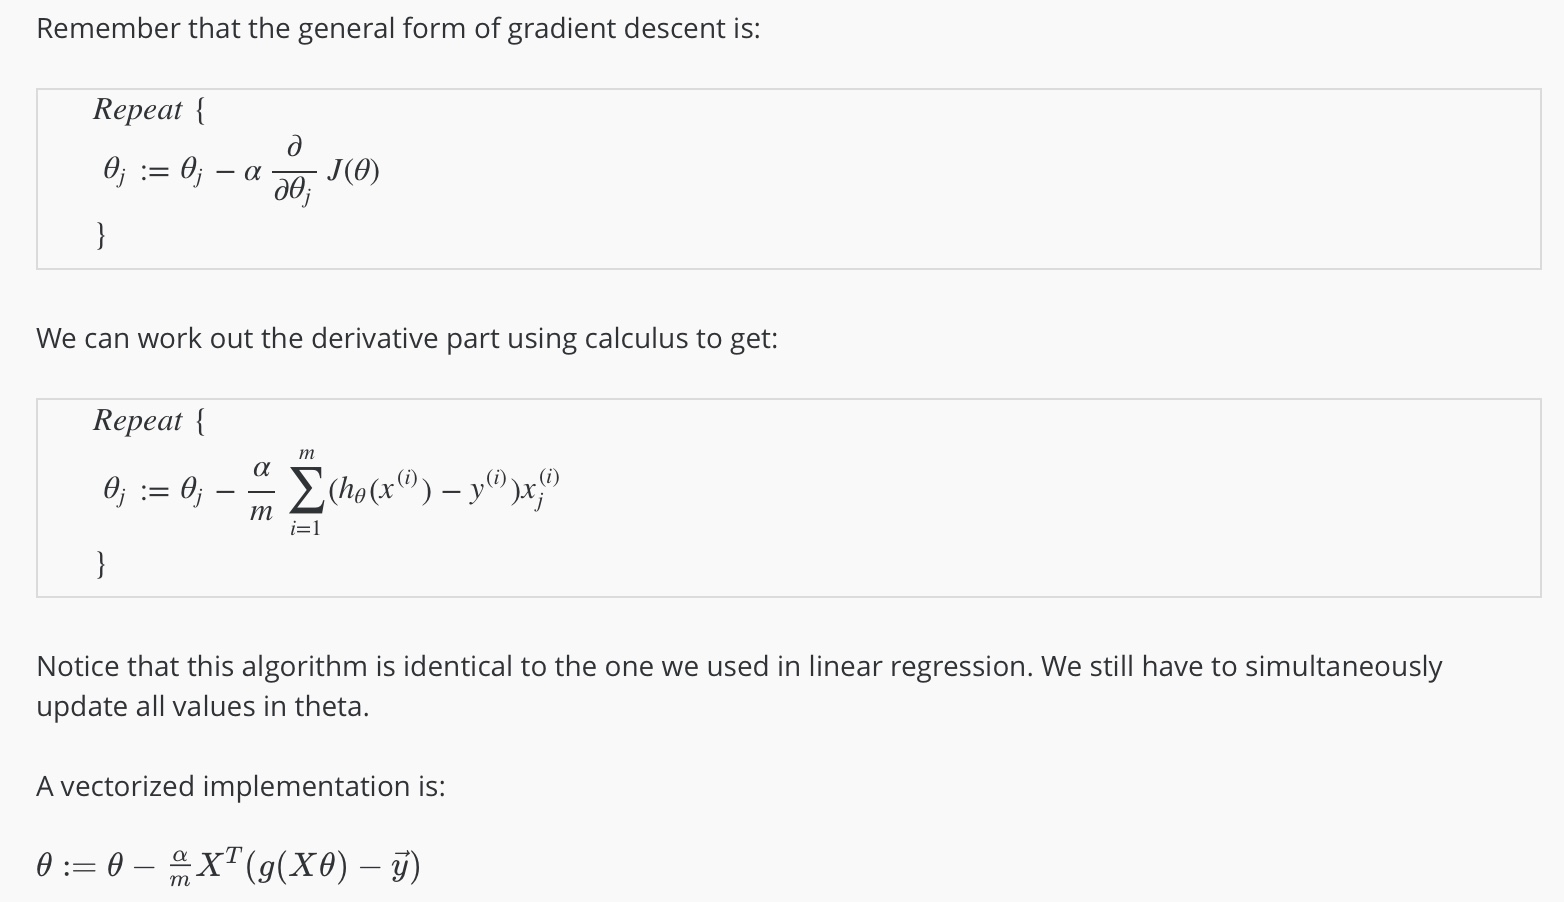
\includegraphics[width=1\textwidth]{./Imagenes/gradDes1}
\end{figure}

\begin{figure}[H]
	\centering
	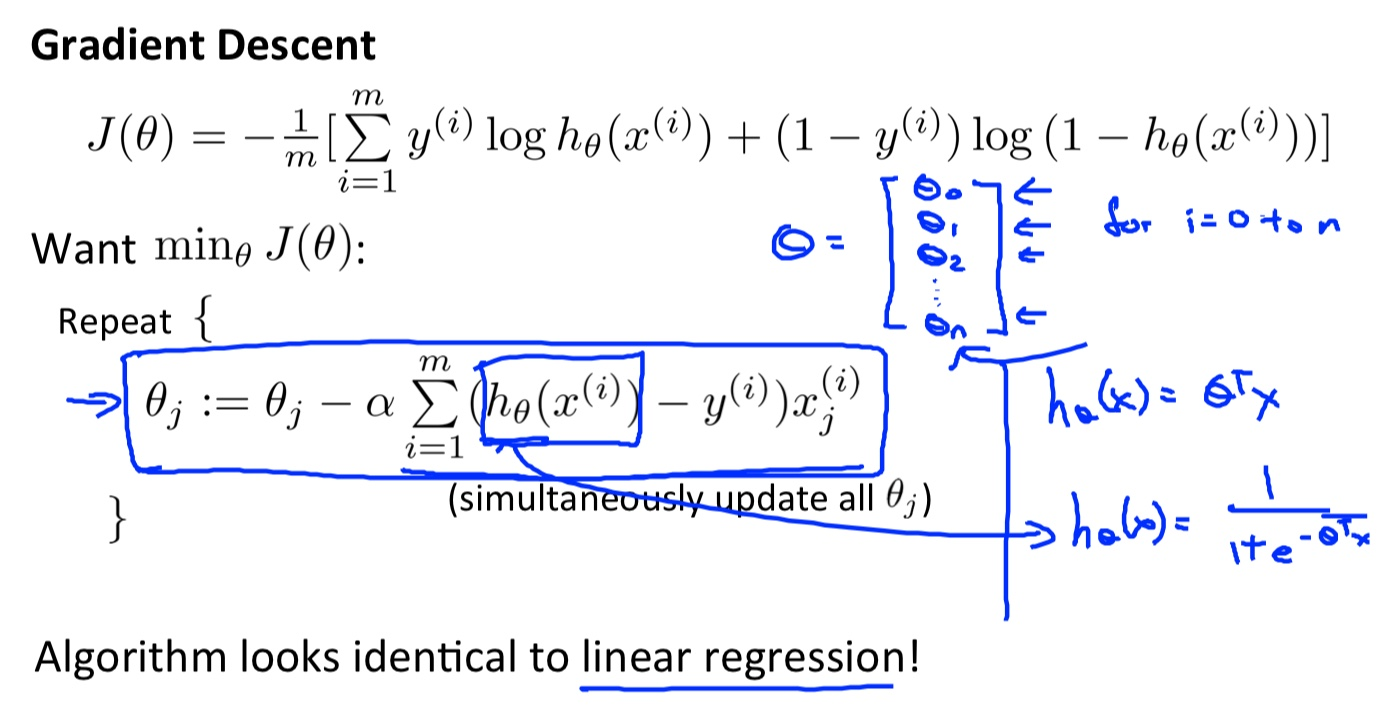
\includegraphics[width=1\textwidth]{./Imagenes/gradDes2}
\end{figure}

\begin{figure}[H]
	\centering
	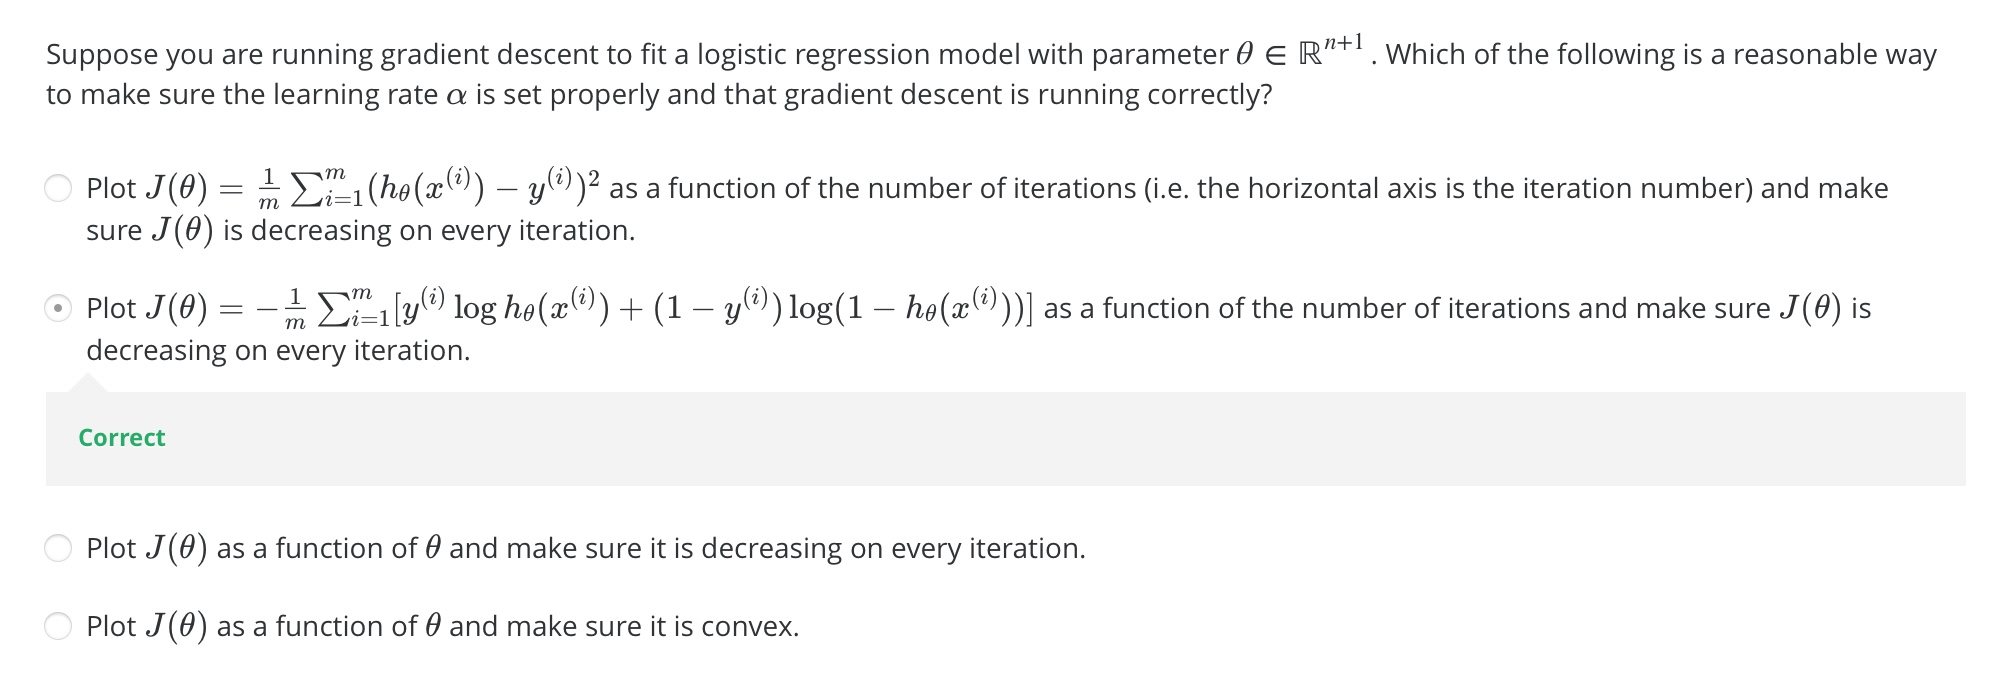
\includegraphics[width=1\textwidth]{./Imagenes/testCostFuncSimple1}
\end{figure}

\begin{figure}[H]
	\centering
	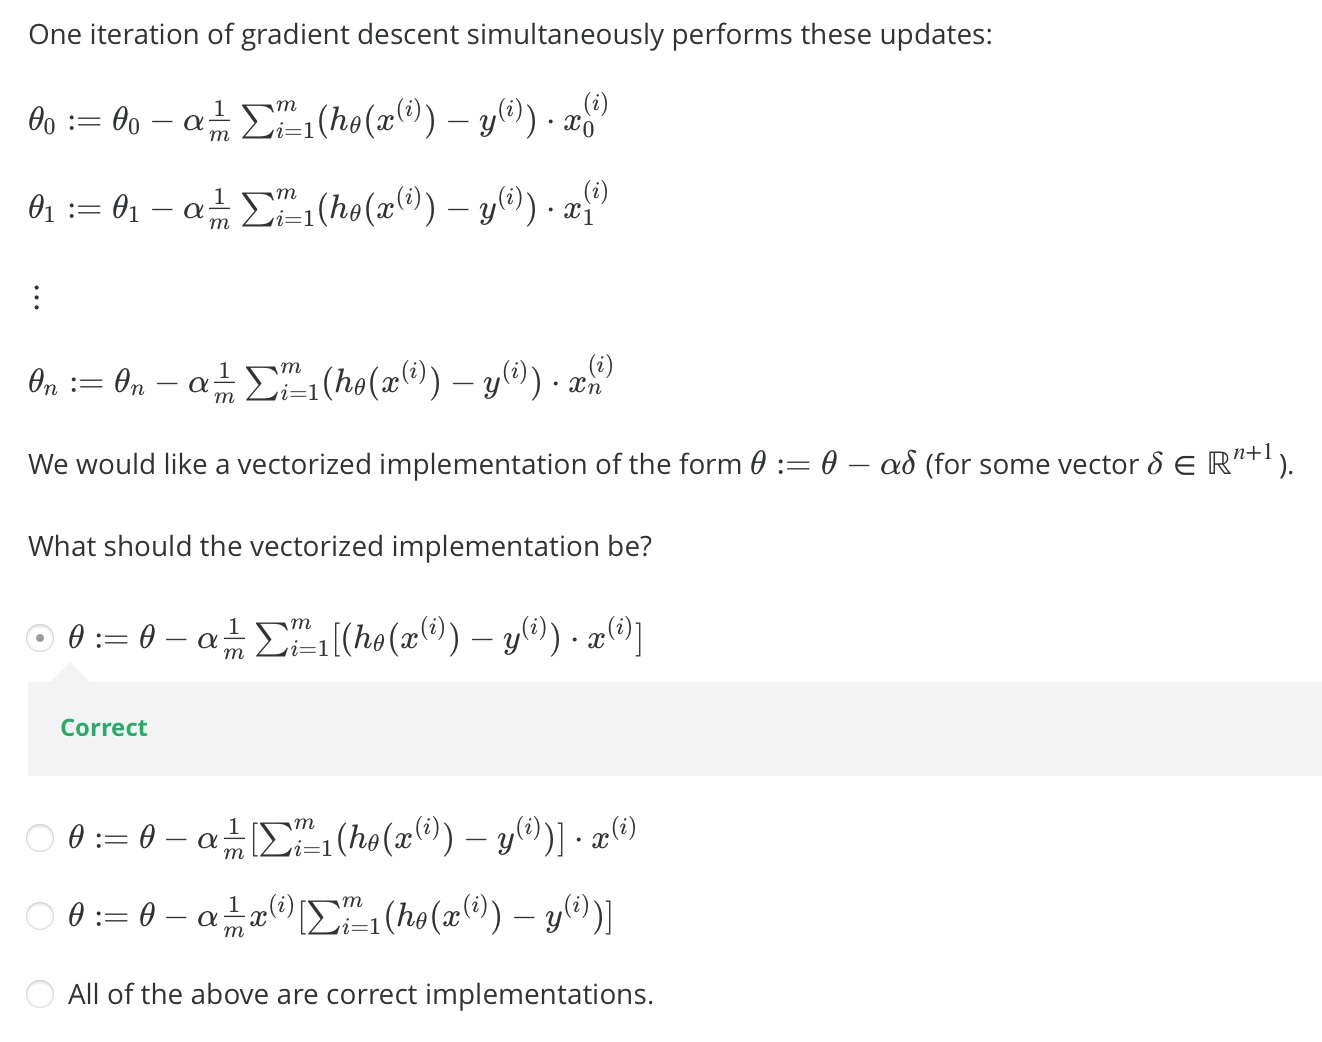
\includegraphics[width=1\textwidth]{./Imagenes/testCostFuncSimple2}
\end{figure}

\newpage

\subsubsection{Advanced optimization}
\begin{figure}[H]
	\centering
	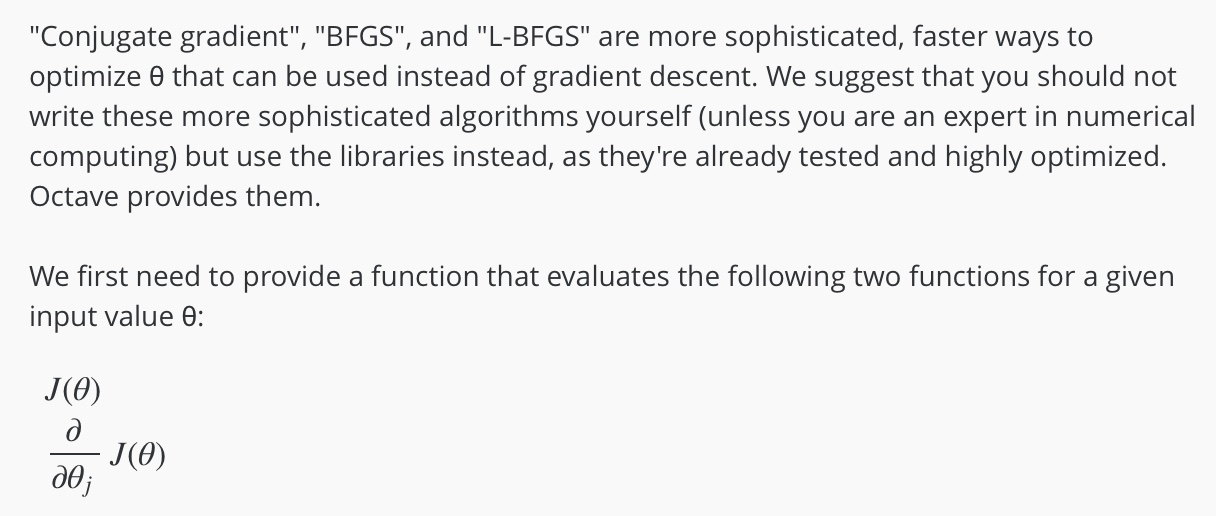
\includegraphics[width=1\textwidth]{./Imagenes/advOpt1}
\end{figure}

\begin{figure}[H]
	\centering
	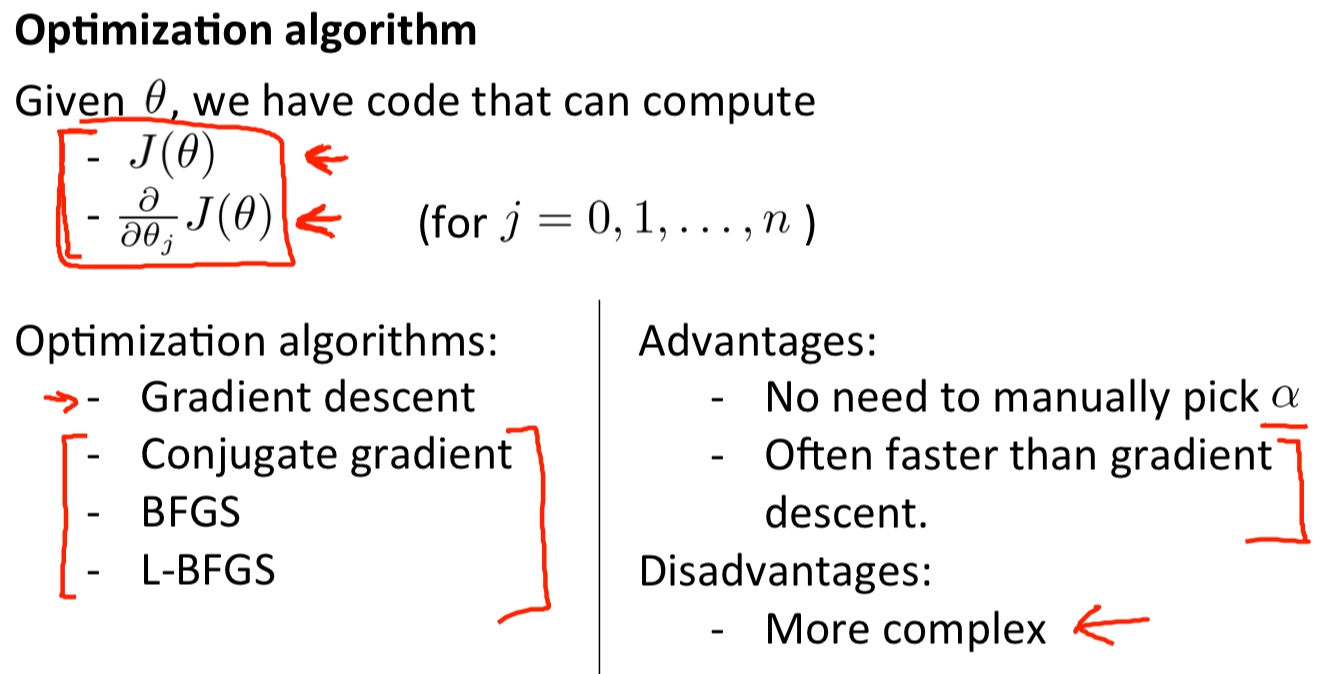
\includegraphics[width=1\textwidth]{./Imagenes/advOpt2}
\end{figure}

\newpage

\subsection{Multiclass classification}
\subsubsection{One-vs-all}

\begin{figure}[H]
	\centering
	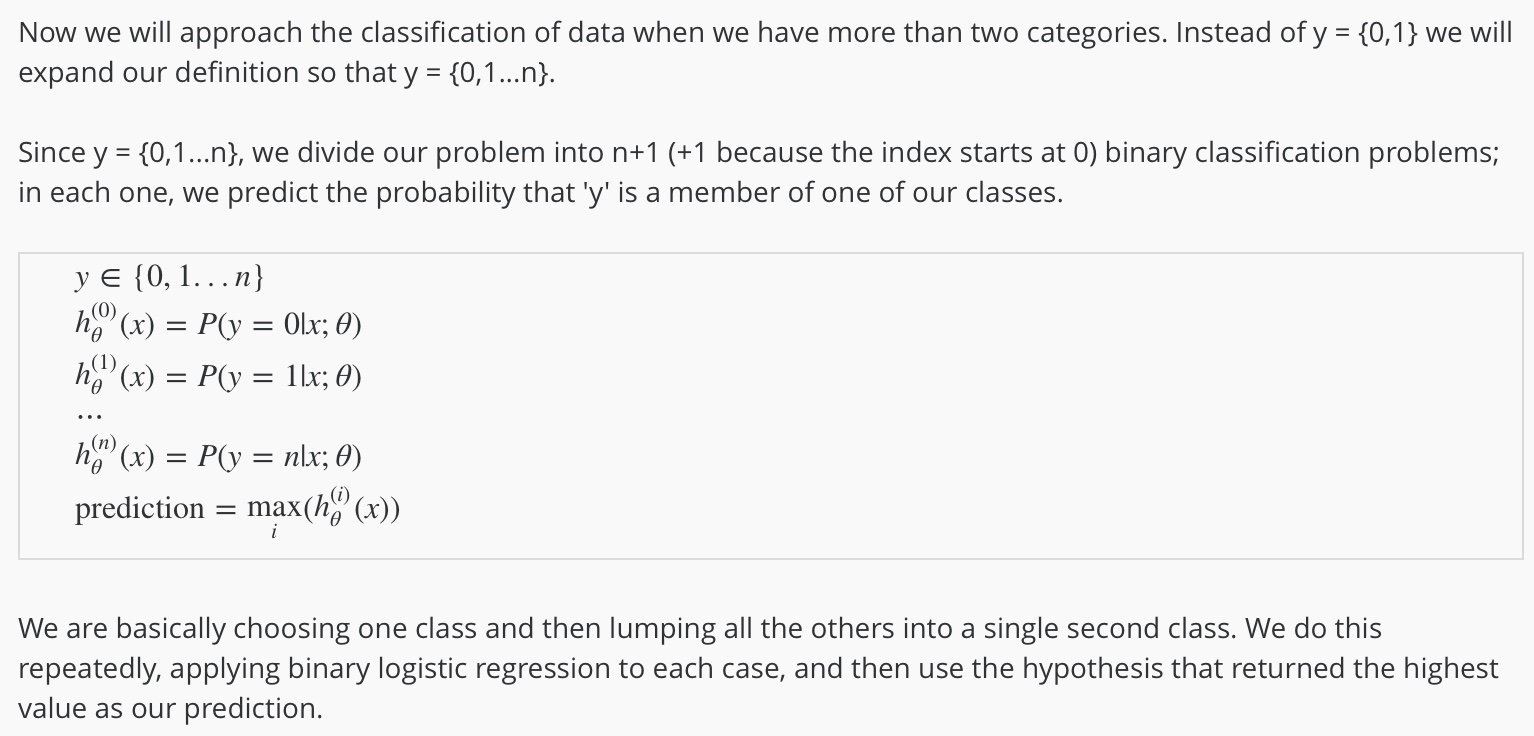
\includegraphics[width=1\textwidth]{./Imagenes/multiClass1}
\end{figure}

\begin{figure}[H]
	\centering
	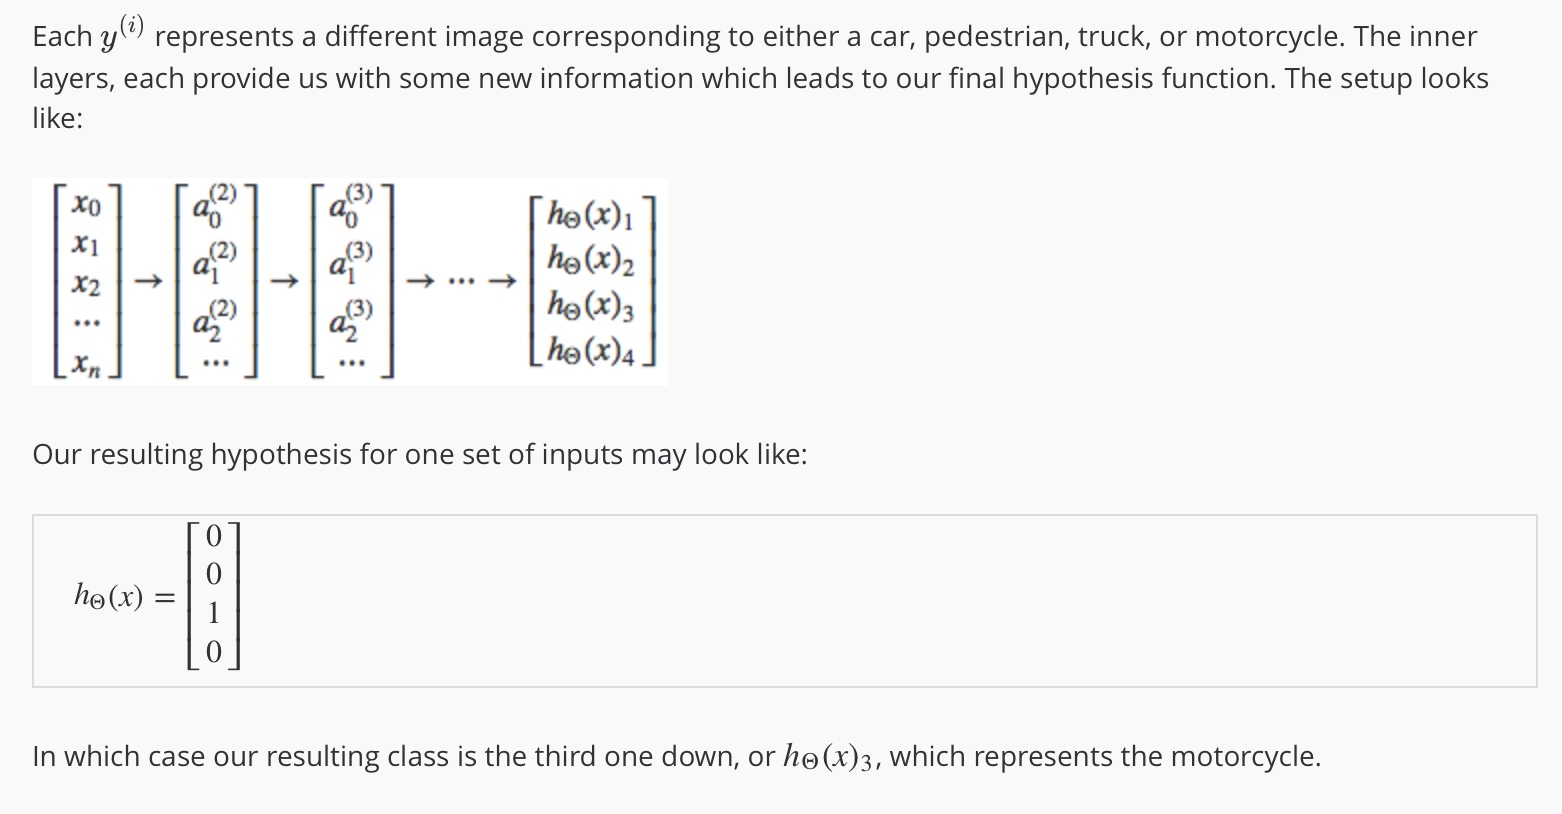
\includegraphics[width=0.85\textwidth]{./Imagenes/multiClass2}
\end{figure}

\begin{figure}[H]
	\centering
	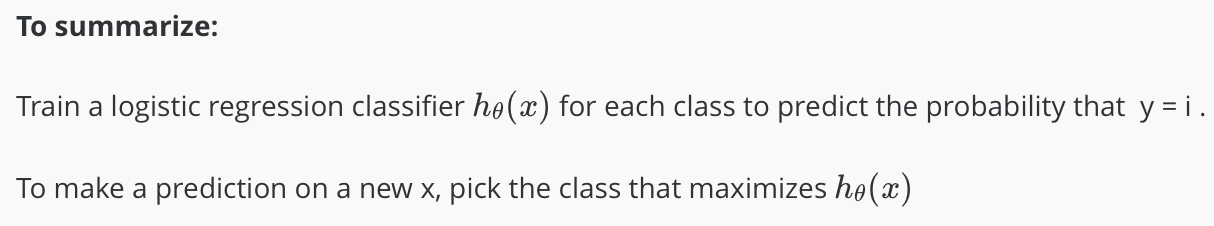
\includegraphics[width=1\textwidth]{./Imagenes/multiClass3}
\end{figure}

\begin{figure}[H]
	\centering
	\includegraphics[width=1\textwidth]{./Imagenes/testMulticlass}
\end{figure}
\newpage

\subsection{Test}

\begin{figure}[H]
\minipage{0.5\textwidth}
  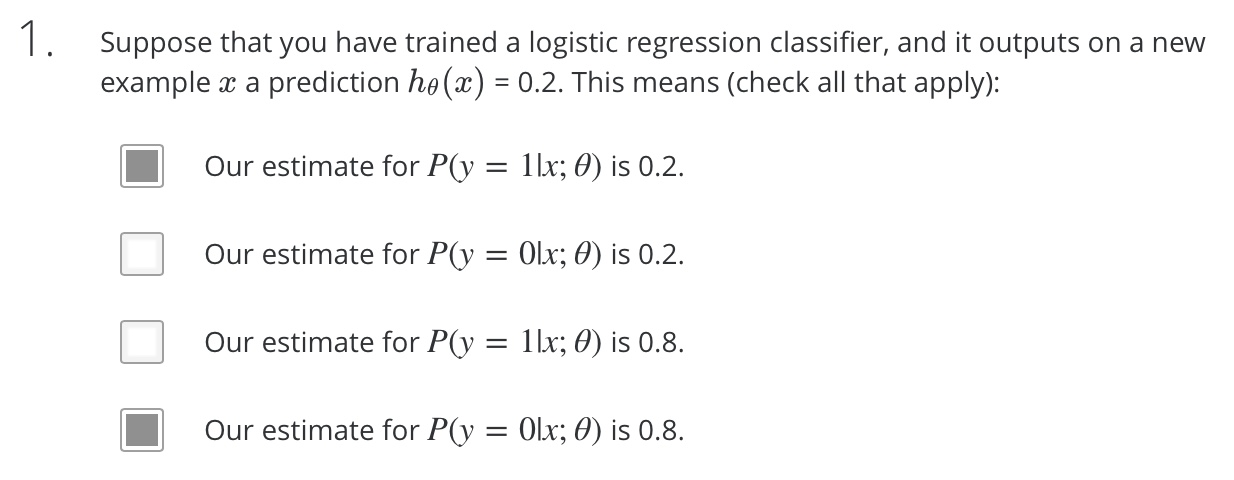
\includegraphics[width=\linewidth]{./Imagenes/testFLogicReg1}
\endminipage\hfill
\minipage{0.5\textwidth}
  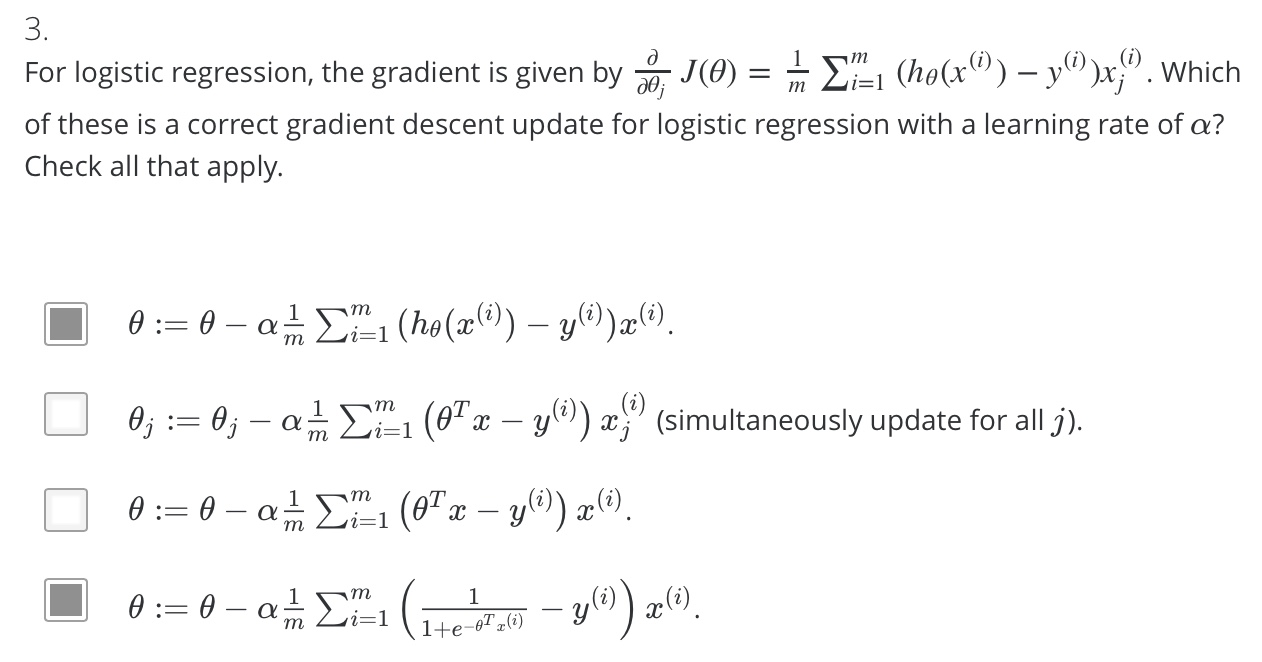
\includegraphics[width=\linewidth]{./Imagenes/testFLogicReg3}
\endminipage\hfill
\end{figure}

\begin{figure}[H]
\minipage{0.5\textwidth}
  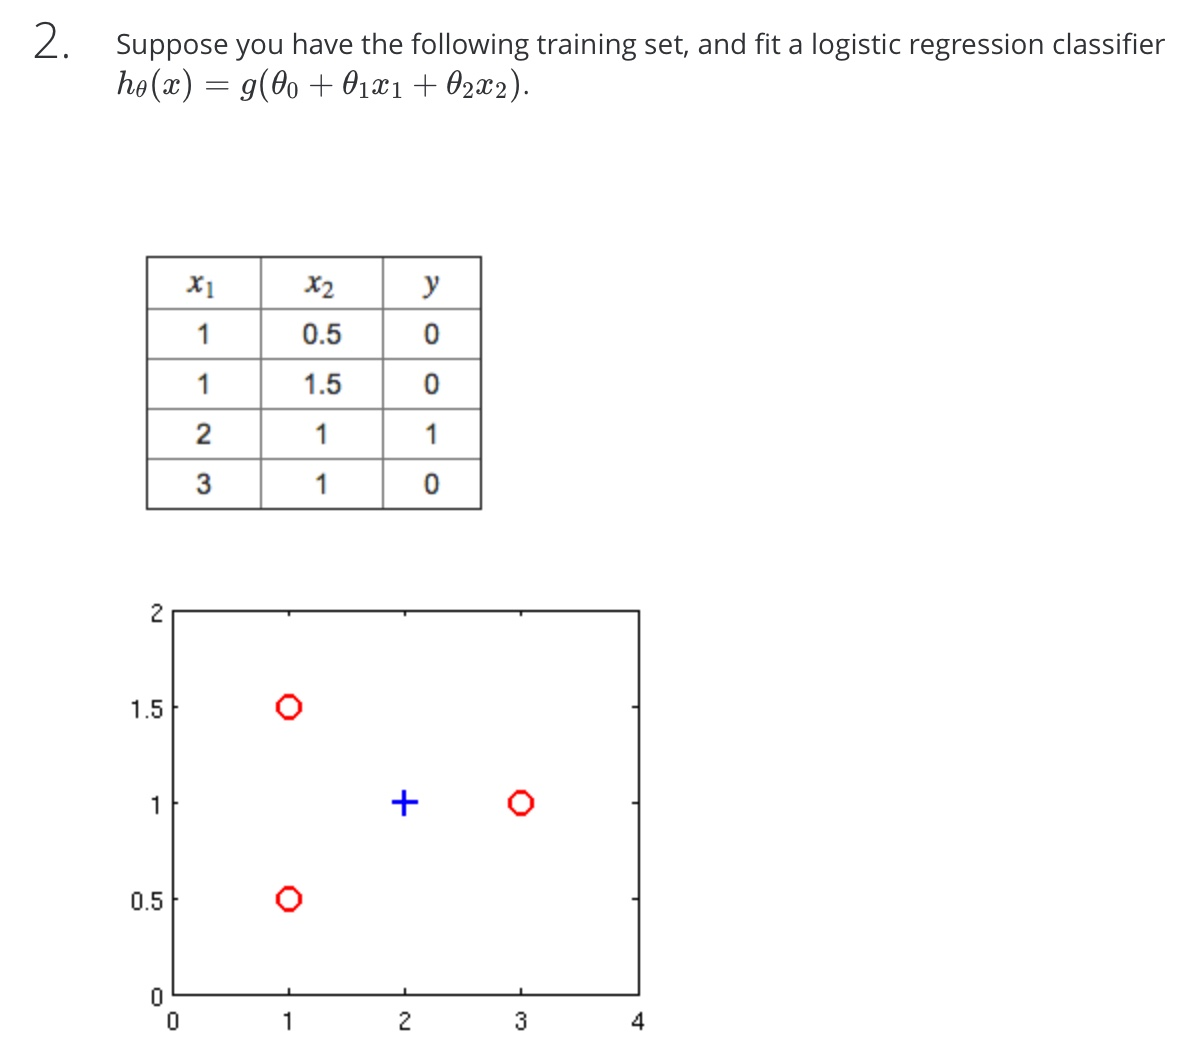
\includegraphics[width=\linewidth]{./Imagenes/testFLogicReg2_1}
\endminipage\hfill
\minipage{0.5\textwidth}
  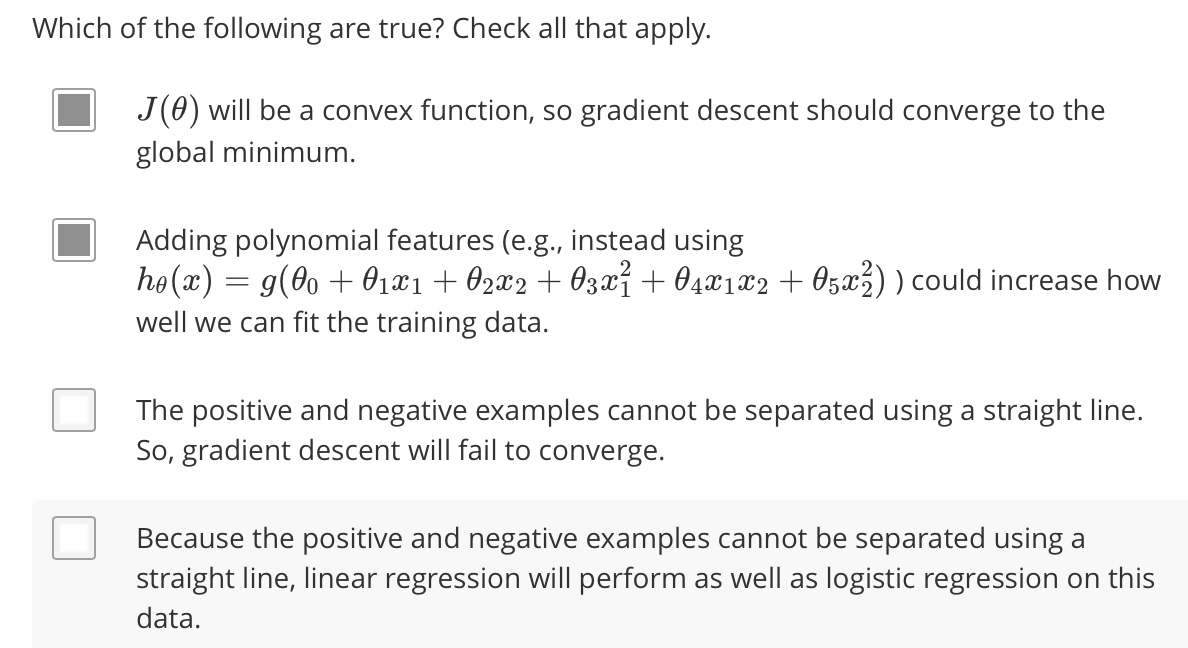
\includegraphics[width=\linewidth]{./Imagenes/testFLogicReg2_2}
\endminipage\hfill
\end{figure}

\begin{figure}[H]
\minipage{0.5\textwidth}
  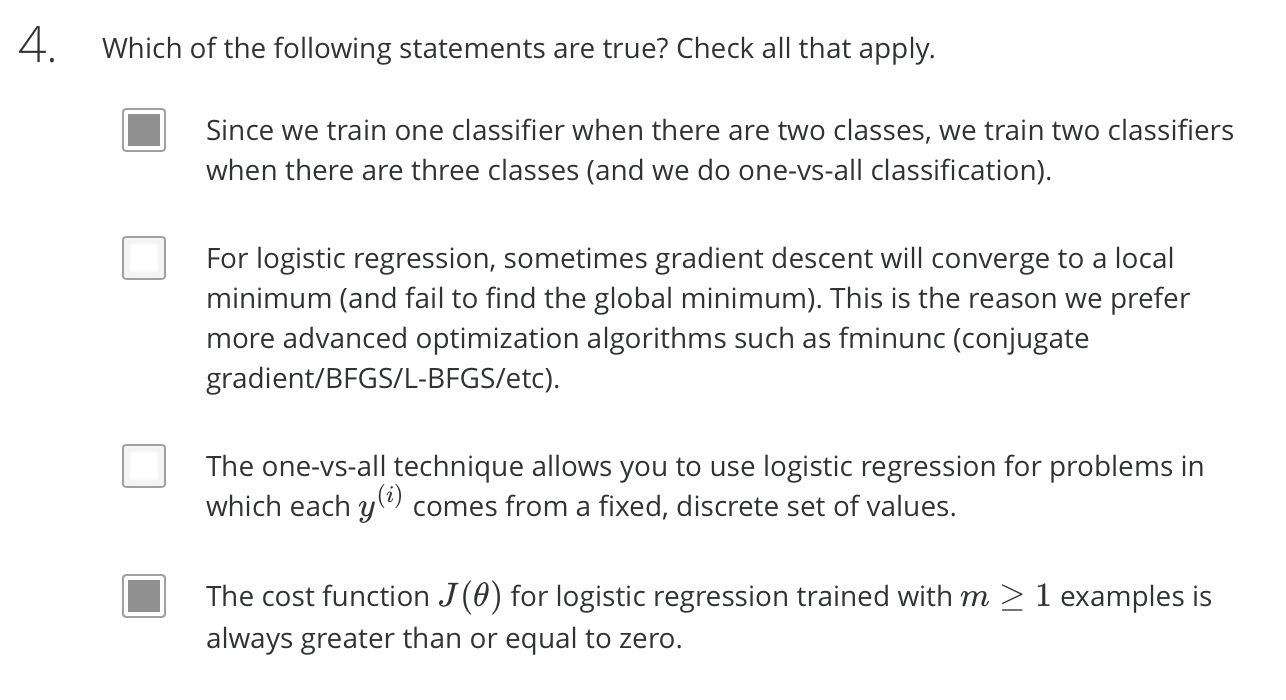
\includegraphics[width=\linewidth]{./Imagenes/testFLogicReg4}
\endminipage\hfill
\minipage{0.5\textwidth}
  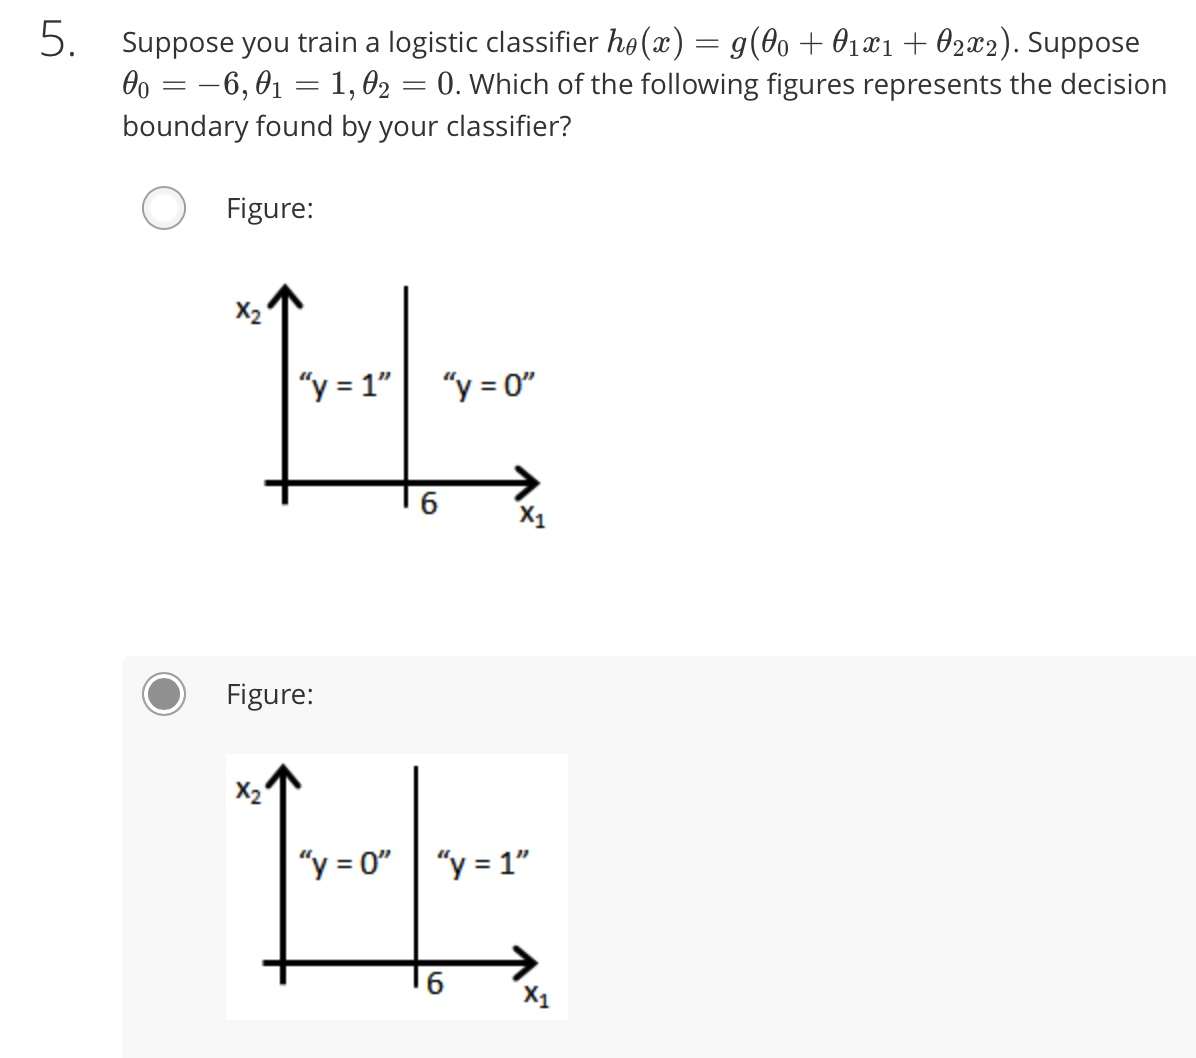
\includegraphics[width=\linewidth]{./Imagenes/testFLogicReg5}
\endminipage\hfill
\end{figure}


\section{Solving the problem of overfitting}
\subsection{The problem of overfitting}

\begin{figure}[H]
	\centering
	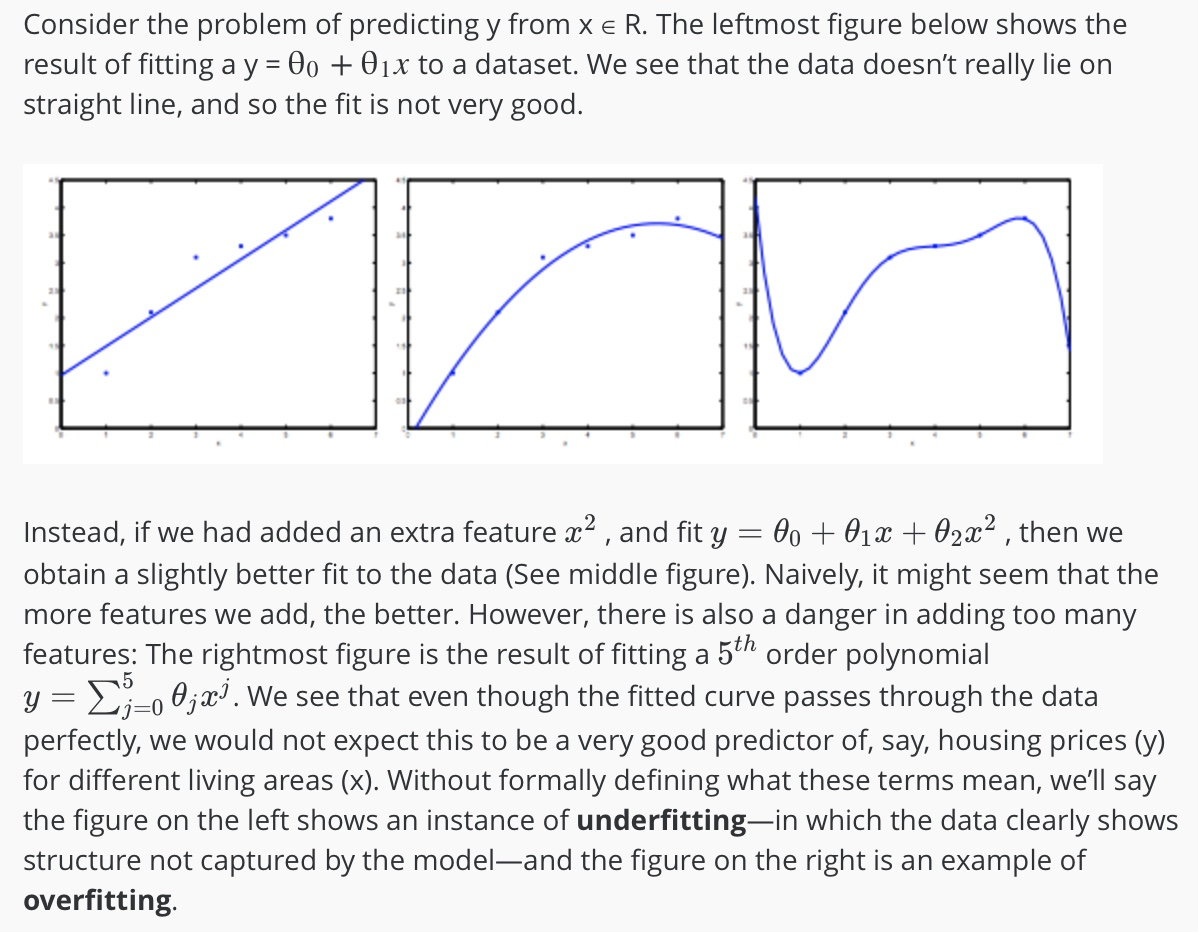
\includegraphics[width=1\textwidth]{./Imagenes/overfit1}
\end{figure}

\begin{figure}[H]
	\centering
	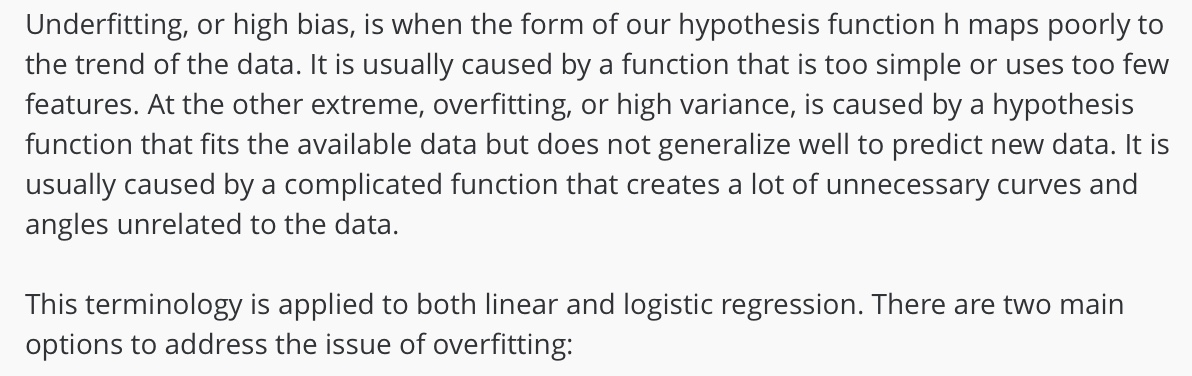
\includegraphics[width=1\textwidth]{./Imagenes/overfit2}
\end{figure}

\begin{figure}[H]
	\centering
	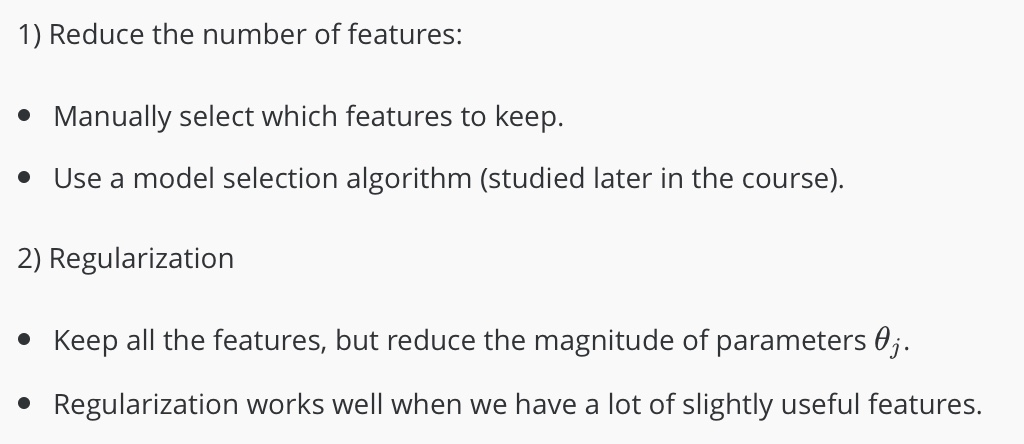
\includegraphics[width=0.8\textwidth]{./Imagenes/overfit3}
\end{figure}

\begin{figure}[H]
	\centering
	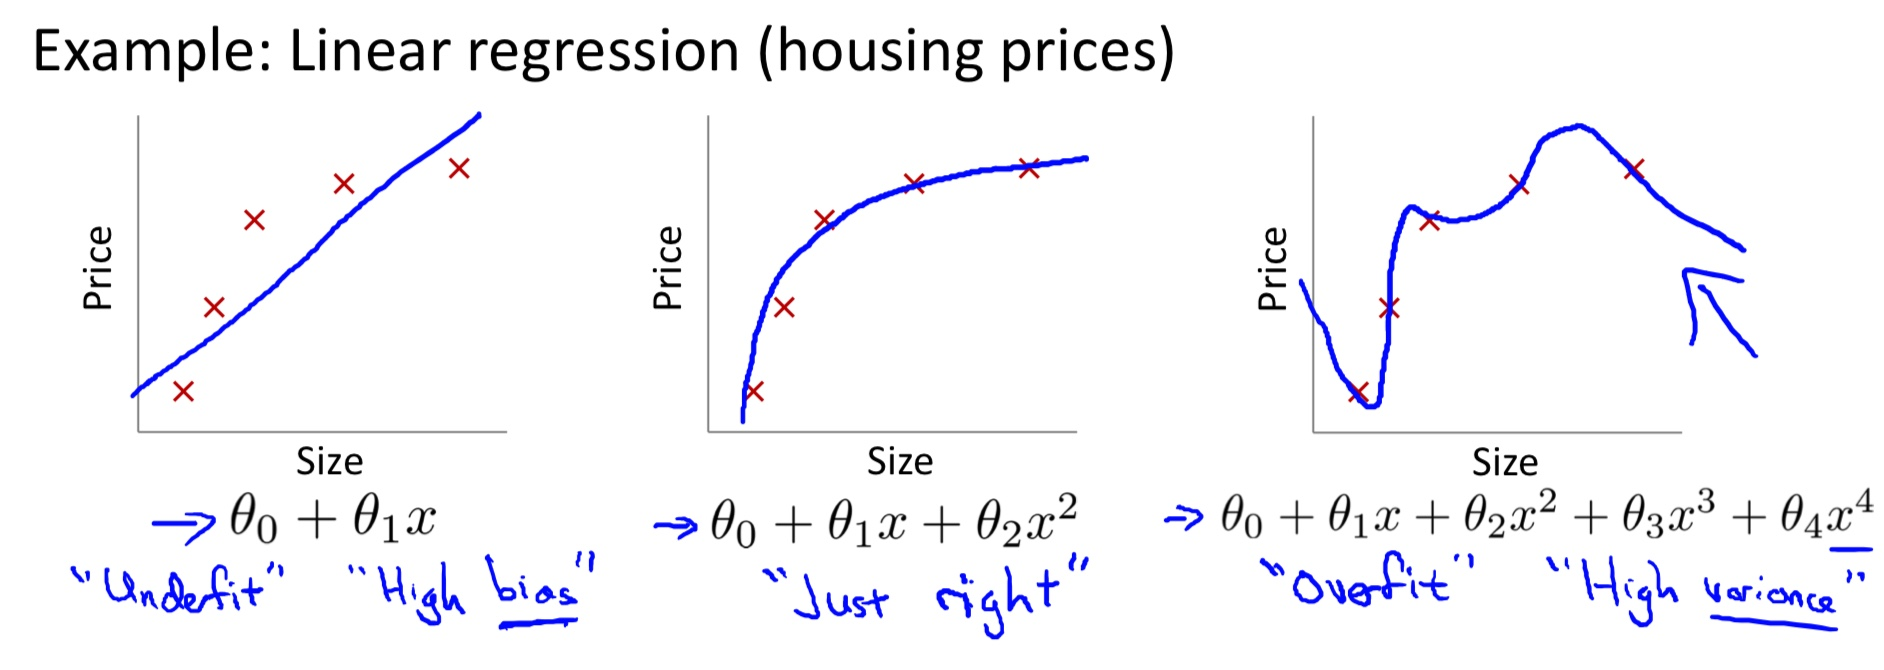
\includegraphics[width=1\textwidth]{./Imagenes/overfit4}
\end{figure}

\begin{figure}[H]
	\centering
	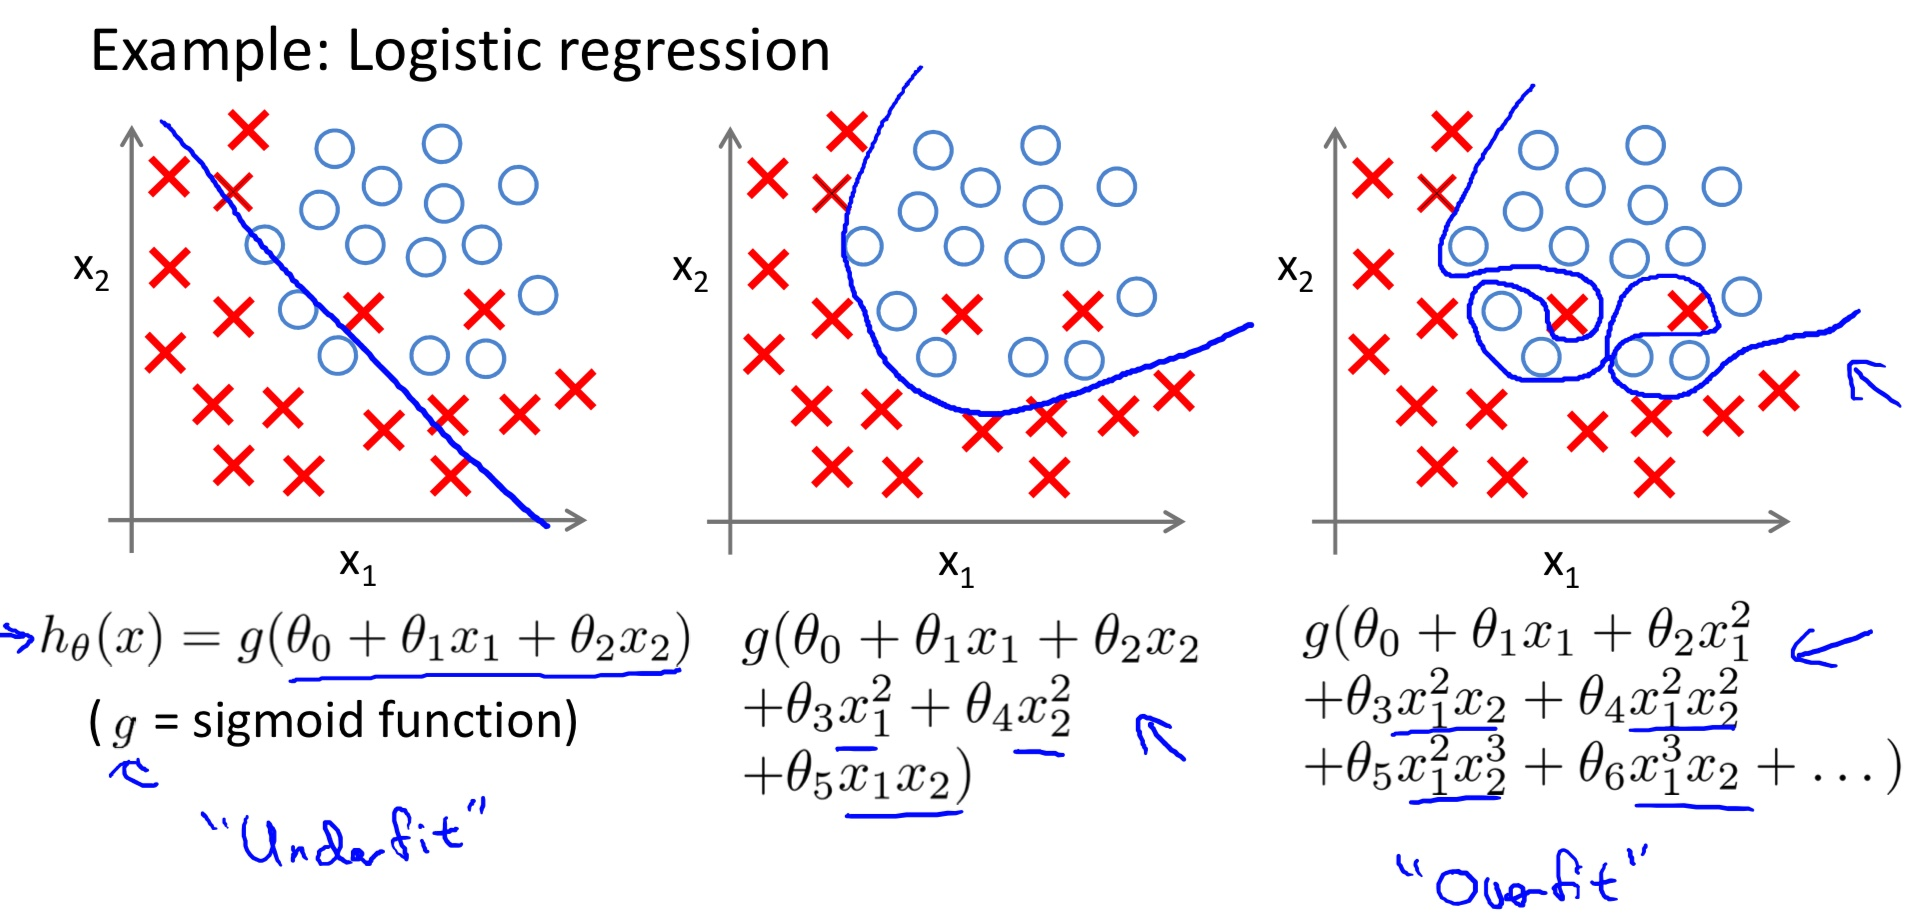
\includegraphics[width=1\textwidth]{./Imagenes/overfit5}
\end{figure}

\subsection{Cost function}
\begin{figure}[H]
	\centering
	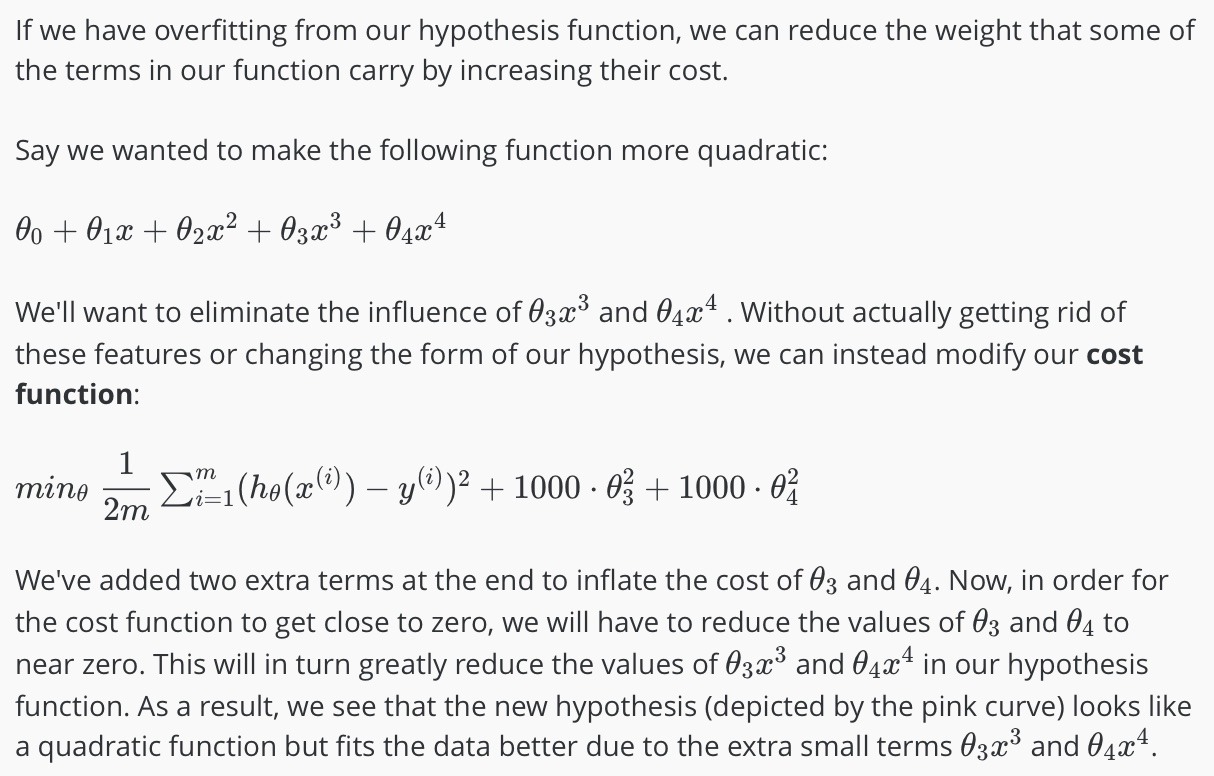
\includegraphics[width=1\textwidth]{./Imagenes/regulCostFunc1}
\end{figure}

\begin{figure}[H]
	\centering
	\includegraphics[width=1\textwidth]{./Imagenes/regulCostFunc2}
\end{figure}

\begin{figure}[H]
	\centering
	\includegraphics[width=0.9\textwidth]{./Imagenes/regulCostFunc3}
\end{figure}

\begin{figure}[H]
	\centering
	\includegraphics[width=0.74\textwidth]{./Imagenes/regulCostFunc4}
\end{figure}

\begin{figure}[H]
	\centering
	\includegraphics[width=0.8\textwidth]{./Imagenes/testRegul}
\end{figure}

\subsection{Regularized linear regression}
\begin{figure}[H]
	\centering
	\includegraphics[width=1\textwidth]{./Imagenes/regulLinearReg1}
\end{figure}

\begin{figure}[H]
	\centering
	\includegraphics[width=0.9\textwidth]{./Imagenes/regulLinearReg2}
\end{figure}

\begin{figure}[H]
	\centering
	\includegraphics[width=1\textwidth]{./Imagenes/regulNormalEq1}
\end{figure}

\begin{figure}[H]
	\centering
	\includegraphics[width=0.9\textwidth]{./Imagenes/regulNormalEq2}
\end{figure}

\begin{figure}[H]
	\centering
	\includegraphics[width=0.9\textwidth]{./Imagenes/testRegulLinear}
\end{figure}
\newpage

\subsection{Regularized logistic regression}
\begin{figure}[H]
	\centering
	\includegraphics[width=1\textwidth]{./Imagenes/regulLogicReg1}
\end{figure}

\begin{figure}[H]
	\centering
	\includegraphics[width=1\textwidth]{./Imagenes/regulLogicReg2}
\end{figure}

\begin{figure}[H]
	\centering
	\includegraphics[width=1\textwidth]{./Imagenes/regulLogicReg3}
\end{figure}

\begin{figure}[H]
	\centering
	\includegraphics[width=1\textwidth]{./Imagenes/regulLogicReg4}
\end{figure}

\begin{figure}[H]
	\centering
	\includegraphics[width=1\textwidth]{./Imagenes/regulLogicReg5}
\end{figure}

\newpage
\subsection{Test}


\begin{figure}[H]
\minipage{0.5\textwidth}
  \includegraphics[width=\linewidth]{./Imagenes/testFRegul1}
\endminipage\hfill
\minipage{0.5\textwidth}
  \includegraphics[width=\linewidth]{./Imagenes/testFRegul2}
\endminipage\hfill
\end{figure}

\begin{figure}[H]
\minipage{0.5\textwidth}
  \includegraphics[width=\linewidth]{./Imagenes/testFRegul3}
\endminipage\hfill
\minipage{0.5\textwidth}
  \includegraphics[width=\linewidth]{./Imagenes/testFRegul4}
\endminipage\hfill
\end{figure}

\begin{figure}[H]
	\centering
	\includegraphics[width=0.7\textwidth]{./Imagenes/testFRegul5}
\end{figure}


\end{document}
